\documentclass[spanish,12pt,titlepage,a4paper]{article}
	\pagestyle{headings}
	\title{\textbf{\Huge{Primeros pasos en Maxima}}}
	\author{\Large{Mario Rodr\'{\i}guez Riotorto}\\
	  \\
	  www.biomates.net\\
	  }
	\setlength{\oddsidemargin}{1cm}
	\setlength{\textwidth}{14cm}
	\setlength{\topmargin}{1.2cm}
	\setlength{\textheight}{20cm}
	\usepackage{graphicx}
	\usepackage{lscape}
	\usepackage[spanish, activeacute]{babel}
	\usepackage{amsfonts}
	\usepackage{latexsym}
	\usepackage{amsmath,amsthm}
	\usepackage{hyperref}
	\usepackage{makeidx}
	\hypersetup{colorlinks, 
           citecolor=black,
           filecolor=black,
           linkcolor=black,
           urlcolor=black,
           pdftex}

	\newcommand{\normal}{\mathcal{N}}
	\newcommand{\N}{\mathbb{N}}
	\newcommand{\Z}{\mathbb{Z}}
	\newcommand{\Q}{\mathbb{Q}}
	\newcommand{\R}{\mathbb{R}}

	\makeindex

	\hyphenation{Ruf-fi-ni e-xer-ci-cios}

%versi'on: 12-06-05

\begin{document}
\maketitle
\newpage
\tableofcontents
\newpage

\bigskip
\begin{quote}
    Copyright \copyright 2005 Mario Rodr'iguez Riotorto.

    Permission is granted to copy, distribute and/or modify this document
    under the terms of the GNU Free Documentation License, Version 1.2
    or any later version published by the Free Software Foundation;
    with no Invariant Sections, no Front-Cover Texts, and no Back-Cover Texts.
    A copy of the license is included in the section entitled "GNU
    Free Documentation License".
\end{quote}
\bigskip

\newpage

\newpage
\section{Introducci'on}

Este es un manual introductorio al entorno de c'alculo simb'olico Maxima, directo sucesor del legendario MACSYMA.

El objetivo del manual es facilitar el acceso a este programa a todas aquellas personas que por vez primera se interesan por 'el.

Maxima es un programa cuyo objeto es la realizaci'on de c'alculos matem'aticos, tanto num'ericos como simb'olicos, capaz de manipular expresiones algebraicas, derivar e integrar funciones y realizar diversos tipos de gr'aficos.

Los or'igenes de Maxima hay que buscarlos a partir del a~no 1967 en el MIT AI Lab (Laboratorio de Inteligencia Artificial del Instituto Tecnol'ogico de Massachussets) como una parte del proyecto MAC (Machine Aided Cognition). El programa recibir'ia por aquel entonces el nombre de Macsyma (MAC's SYmbolic MAnipulator), del cual el MIT mandar'ia una copia en 1982 al DOE (US Department Of Energy), uno de los organismos que aportaron los fondos econ'omicos para el desarrollo del proyecto; esta primera versi'on se la conoce como DOE-Macsyma. Posteriormente, el DOE concede la licencia de explotaci'on del programa a la empresa Symbolics, que sigue desarrollando el proyecto durante unos a~nos. En 1992 el programa es adquirido por una empresa que se llamar'ia precisamente Macsyma Inc, y el programa ir'ia perdiendo fuelle progresivamente ante la presencia en el mercado de otros programas similares como Maple o Mathematica, ambos los dos inspirados en sus or'igenes por el propio Macsyma.

Pero ocurrieron dos historias paralelas. Desde el a~no 1982, y hasta su fallecimiento en el 2001, William Schelter en la Universidad de Texas mantuvo una versi'on de este programa adaptada al est'andar Common Lisp, la cual ya se conoc'ia con el nombre de Maxima para diferenciarla de la versi'on comercial. En el a~no 1998 Schelter consigui'o del DOE permiso para distribuir Maxima bajo la licencia GNU-GPL (www.gnu.org); con este paso, muchas m'as personas empezaron a dirigir su mirada hacia Maxima, justo en el momento en el que la versi'on comercial estaba pr'acticamente muerta. Actualmente, el proyecto est'a siendo liderado por un grupo de investigadores originarios de varios pa'ises, tanto del entorno universitario como empresarial, asistidos y ayudados por otras muchas personas interesadas en Maxima y que mantienen un cauce de comunicaci'on a trav'es de una lista de correo (maxima.sourceforge.net/maximalist.html).

Puesto que Maxima se distribuye bajo la licencia GNU-GPL, tanto el c'odigo fuente como los manuales son de libre acceso a trav'es de la p'agina web del proyecto (maxima.sourceforge.net).

Como profesor de matem'aticas, no me resisto a traducir unas l'ineas del cap'itulo introductorio del manual oficial del programa:

\begin{quote}
Aquellos que se presten a utilizar el ordenador para hacer matem'aticas, particularmente los estudiantes, deben estar sobre aviso de que estos entornos no son sustitutos del trabajo manual con las ecuaciones ni del esfuerzo por comprender los conceptos. Estos medios no ayudan a formar la intuici'on matem'atica ni a reforzar los conocimientos fundamentales... No se debe utilizar el ordenador como un sustituto de la formaci'on b'asica.

Sin embargo, el dominio del ordenador y de las herramientas matem'aticas computacionales son cruciales a la hora de abordar el gran n'umero de problemas que no pueden ser resueltos simplemente con l'apiz y papel. En muchos casos, problemas que tardar'ian a~nos en ser resueltos de forma manual pueden ser solventados en cuesti'on de segundos con un ordenador... Adem'as, en caso de error, su correcci'on ser'a m'as r'apida y sencilla volviendo a ejecutar un c'odigo ya escrito, pero convenientemente modificado para subsanar el fallo.

Si bien el ordenador puede corregir los errores humanos, el humano por su parte tampoco debe confiar en el ordenador de forma incuestionable. Todos estos sistemas tienen sus l'imites y cuando 'estos son alcanzados, es posible obtener respuestas incorrectas... As'i pues, no se puede uno olvidar de revisar los resultados que se obtienen. El ordenador no siempre dice la verdad, y si la dice, quiz'as no sea completa.
\end{quote}

\begin{flushright}
\emph{Ferrol-A Coru~na}
\end{flushright}


\newpage
\section{Instalaci'on}

Es posible tener operativo Maxima tanto en Linux como en Windows. La informaci'on para la instalaci'on en estos dos sistemas se puede encontrar en la p'agina \emph{web} del proyecto.

En lo que a Linux se refiere, el paquete b'asico permite tener operativo Maxima en el entorno de la consola de texto, Figura~\ref{fig:consola}, pero tambi'en es posible la instalaci'on de m'odulos o programas adicionales que permitan la utilizaci'on del programa a trav'es de un entorno gr'afico; aqu'i se pueden barajar varias opciones: xmaxima, Figura~\ref{fig:tcl}, basado en Tcl-Tk y descargable desde la propia p'agina del proyecto Maxima; wxmaxima (wxmaxima.sourceforge.net), Figura~\ref{fig:wxmaxima}, basado en wxWidgets y de aparici'on m'as reciente; tambi'en existe la posibilidad de acceder a Maxima desde una sesi'on del editor de texto WYSIWYG TeXmacs (www.texmacs.org), Figura~\ref{fig:texmacs}, que al hacer uso de las fuentes \TeX (www.tug.org/teTeX) aumenta considerablemente la calidad en la impresi'on de f'ormulas y expresiones matem'aticas. Un programa adicional que no debe faltar es gnuplot (www.gnuplot.info) para la representaci'on de gr'aficos en 2D y 3D. Todos estos programas se pueden descargar gratuitamente desde Internet. Para la instalaci'on de estos programas l'ease la documentaci'on correspondiente a cada caso.

Tambi'en, y para los m'as valientes, se puede descargar el c'odigo fuente y compilarlo, para lo que ser'a necesario tener operativo un entorno Lisp en la m'aquina, como GCL (www.gnu.org/software/gcl), CLISP (clisp.cons.org) o CMUCL (www.cons.org/cmucl).

En cuanto a Windows, tambi'en desde la p'agina del proyecto se puede descargar un ejecutable que instala  xmaxima, con un aspecto similar al de la Figura~\ref{fig:tcl}. Si se prefiere wxmaxima, una vez instalado el paquete anterior, se har'a uso del ejecutable para este sistema operativo que se encontrar'a en el sitio wxmaxima.sourceforge.net. 

\begin{figure}
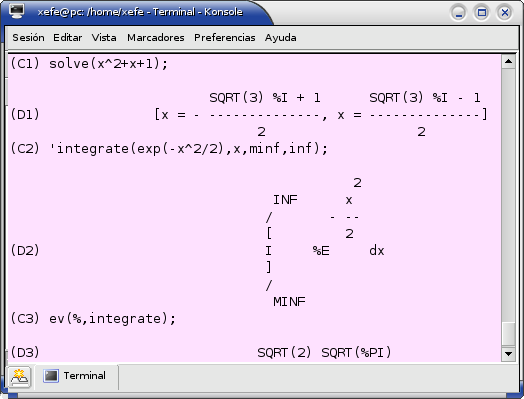
\includegraphics[angle=90]{maxima.png}
\caption{Maxima operando en la consola de texto.}
\label{fig:consola}
\end{figure}


\begin{figure}
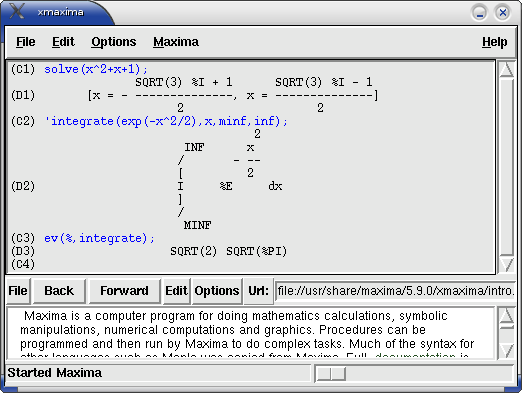
\includegraphics[angle=90]{xmaxima.png}
\caption{xmaxima: Maxima trabajando en el entorno gr'afico Tcl-Tk.}
\label{fig:tcl}
\end{figure}


\begin{figure}
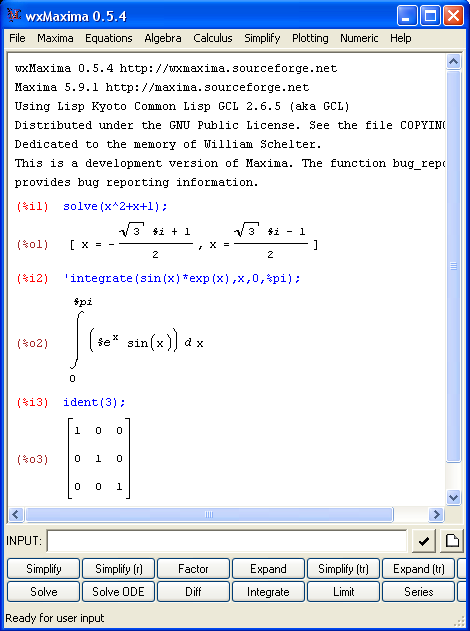
\includegraphics[]{wxmaxima.png}
\caption{wxmaxima: Maxima ejecut'andose en Windows.}
\label{fig:wxmaxima}
\end{figure}


\begin{figure}
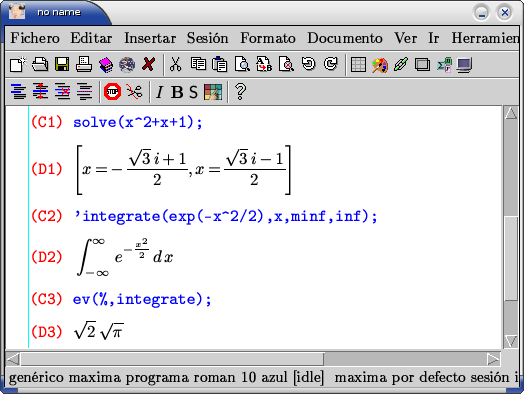
\includegraphics[angle=90]{texmacs.png}
\caption{Maxima trabajando en TeXmacs.}
\label{fig:texmacs}
\end{figure}




\newpage
\section{Primera sesi'on con Maxima}

Una vez accedemos a Maxima, lo primero que vamos a ver ser'a la siguiente informaci'on:
\begin{verbatim}
Maxima 5.9.2 http://maxima.sourceforge.net
Using Lisp CLISP 2.33.2 (2004-06-02)
Distributed under the GNU Public License. See the file COPYING.
Dedicated to the memory of William Schelter.
This is a development version of Maxima. The function bug_report()
provides bug reporting information.
(%i1)
\end{verbatim}

Tras la informaci'on sobre la licencia, por supuesto GNU-GPL, nos informa sobre la versi'on con la que estamos trabajando y la p'agina \emph{web} del proyecto. A continuaci'on, muy importante, aparece el indicador \verb|(%i1)| esperando nuestra primera pregunta. Si queremos calcular una simple suma tecleamos la operaci'on deseada seguida de un punto y coma (\verb|;|)\index{1@; (punto y coma)} y una pulsaci'on de la tecla retorno
\begin{verbatim}
(%i1) 45 + 23;
\end{verbatim}
a lo que Maxima nos contestar'a
\begin{verbatim}
(%o1)                        68
(%i2)
\end{verbatim}
indicando \verb|(%i2)| que Maxima espera nuestra segunda instrucci'on.

El punto y coma act'ua tambi'en como un separador cuando escribimos varias instrucciones en un mismos rengl'on. Nuestra siguiente operaci'on consistir'a en asignar el valor 34578 a la variable \verb|x| y el 984003 a la \verb|y|, solicitando luego su producto,
\begin{verbatim}
(%i2) x:34578; y:984003; x*y;
(%o2)                     34578
(%o3)                     984003
(%o4)                  34024855734
(%i5)
\end{verbatim}
conviene prestar atenci'on al hecho de que la asignaci'on de un valor a una variable se hace con los dos puntos, no con el signo de igualdad, que se reserva para las ecuaciones.

Es posible que no deseemos los resultados intermedios que Maxima va calculando o, como en este caso, las asignaciones a las variables que va haciendo; en tales situaciones conviene hacer uso del delimitador \verb|$|\index{3@\$}, que no devuelve a la consola los resultados que va calculando. Repitiendo el c'alculo de la forma 
\begin{verbatim}
(%i5) x:34578$ y:984003$ x*y;
(%o7)                  34024855734
\end{verbatim}
podemos conseguir una salida m'as limpia. Las asignaciones a variables se mantienen activas mientras dure la sesi'on con Maxima, por lo que podemos restar las variables \verb|x| e \verb|y| anteriores
\begin{verbatim}
(%i8) x-y;
(%o8)                    - 949425
\end{verbatim}
Esto tiene un riesgo; si queremos resolver la ecuaci'on $x^2-3x+1=0$,
\begin{verbatim}
(%i9) solve(x^2-3*x+1=0,x);
A number was found where a variable was expected -`solve'
 -- an error.  Quitting.  To debug this try debugmode(true);
\end{verbatim}
nos devuelve un mensaje de error, ya que donde se supone que hay una inc'ognita, lo que realmente encuentra es un n'umero, en este caso 34578. El problema se resuelve vaciando el contenido de la variable \verb|x| mediante la funci'on \verb|kill|\index{kill},
\begin{verbatim}
(%i10) kill(x)$
(%i11) solve(x^2-3*x+1=0,x);
                   sqrt(5) - 3      sqrt(5) + 3
(%o11)      [x = - -----------, x = -----------]
                        2                2
\end{verbatim}
luego las soluciones de la ecuaci'on forman el conjunto $\{-\frac{\sqrt{5}-3}{2}, \frac{\sqrt{5}+3}{2}\}$. Ya vemos que en Maxima la ra'iz cuadrada se calcula con la funci'on \verb|sqrt|\index{sqrt}.

Las etiquetas \verb|(%ix)|\index{7@\%ix} y \verb|(%ox)|\index{8@\%ox}, siendo \verb|x| un n'umero entero, pueden ser utilizadas a lo largo de una sesi'on a fin de evitar tener que volver a escribir expresiones; as'i, si queremos calcular el cociente $\frac{x y}/{x-y}$, con $x=34578$ y $y=984003$, podemos aprovechar los resultados \verb|(%o7)| y \verb|(%o8)| y hacer
\begin{verbatim}
(%i12) %o7/%o8;
                         11341618578
(%o12)                 - -----------
                           316475
\end{verbatim}

Las etiquetas que indican las entradas y salidas pueden ser modificadas a voluntad haciendo uso de las variables \verb|inchar|\index{inchar} y \verb|outchar|\index{outchar},
\begin{verbatim}
(%i13) inchar;
(%o13)                       %i
(%i14) outchar;
(%o14)                       %o
(%i15) inchar: "menda";
(%o15)                     menda
(menda15) outchar: "lerenda";
(lerenda15)               lerenda
(menda16) 2+6;
(lerenda16)                  8
(menda17) inchar:"%i"$ outchar:"%o"$
(%i17)
\end{verbatim}

En caso de que se pretenda realizar nuevamente un c'alculo ya indicado deber'a escribirse dos comillas simples (\verb|''|)\index{5@''}, no comilla doble, junto con la etiqueta de la instrucci'on deseada
\begin{verbatim}
(%i18) ''%i9;
(%o18)                   x - 984003
\end{verbatim}
Obs'ervese que al haber dejado a \verb|x| sin valor num'erico, ahora el resultado es otro. Cuando se quiera hacer referencia al 'ultimo resultado calculado por Maxima puede ser m'as sencillo hacer uso del s'imbolo  \verb|%|\index{6@\%}, de forma que si queremos restarle la \verb|x| a la 'ultima expresi'on podemos hacer
\begin{verbatim}
(%i19) %-x;
(%o19)                    - 984003
\end{verbatim}

Ciertas constantes matem'aticas de uso frecuente tienen un s'imbolo especial en Maxima: la base de los logaritmos naturales ($e$), el cociente entre la longitud de una circunferencia y su di'ametro ($\pi$), la unidad imaginaria ($i=\sqrt{-1}$) y la constante de Euler-Mascheroni ($\gamma=-\int_0^\infty e^{-x} \ln x dx$), se representar'an por \verb|%e|\index{9@\%e}, \verb|%pi|\index{11@\%pi}, \verb|%i|\index{10@\%i} y \verb|%gamma|\index{12@\%gamma}, respectivamente.

Es muy sencillo solicitar a Maxima que nos informe sobre alguna funci'on de su lenguaje; la t'ecnica nos servir'a para ampliar informaci'on sobre cualquier instrucci'on a la que se haga referencia en este manual, por ejemplo,
\begin{verbatim}
(%i20) describe(sqrt);

 0: isqrt :(maxima.info)Definitions for Operators.
 1: sqrt :Definitions for Operators.
 2: sqrtdispflag :Definitions for Operators.
Enter space-separated numbers, `all' or `none': 1

Info from file /usr/local/info/maxima.info:
 - Function: sqrt (<x>)
     The square root of <x>. It is represented internally by
     `<x>^(1/2)'.  See also `rootscontract'.

     `radexpand' if `true' will cause nth roots of factors of a product
     which are powers of n to be pulled outside of the radical, e.g.
     `sqrt(16*x^2)' will become `4*x' only if `radexpand' is `true'.

(%o20)                     false
\end{verbatim}
Inicialmente muestra un sencillo men'u en el que debemos seleccionar qu'e informaci'on concreta deseamos; en esta ocasi'on se opt'o por \verb|1| que es el n'umero asociado a la funci'on que interesaba.

A fin de no perder los resultados de una sesi'on con Maxima, quiz'as con el objeto de continuar el trabajo en pr'oximas jornadas, podemos guardar en un archivo aquellos valores que nos puedan interesar; supongamos que necesitamos almacenar el contenido de la variable \verb|y|, tal como lo definimos en la entrada \verb|(%i5)|, as'i como el resultado de la salida 
\verb|(%o11)|, junto con la instrucci'on que la gener'o, la entrada \verb|(%i11)|,
\begin{verbatim}
(%i21) save("mi.sesion",y,resultado=%o11,ecuacion=%i11)$
\end{verbatim}
Compru'ebese que el primer argumento de \verb|save|\index{save} es el nombre del archivo, junto con su ruta si se considera necesario, que la variable \verb|y| se escribe tal cual, pero que a las referencias de las entradas y salidas deben ir acompa~nadas de un nombre que las haga posteriormente reconocibles.

Por 'ultimo, la forma correcta de abandonar la sesi'on de Maxima es mediante
\index{quit}\begin{verbatim}
(%i22) quit();
\end{verbatim}

Abramos ahora una nueva sesi'on con Maxima y carguemos en memoria los resultados de la anterior sesi'on,
\index{load}\begin{verbatim}
(%i1) load("mi.sesion")$
(%i2) y;
(%o2)                      984003
(%i3) ecuacion;
                        2
(%o3)            solve(x  - 3 x + 1 = 0, x)
(%i4) resultado;
                   sqrt(5) - 3      sqrt(5) + 3
(%o4)       [x = - -----------, x = -----------]
                        2                2
\end{verbatim}

Si ahora quisi'eramos recalcular las soluciones de la ecuaci'on, modific'andola previamente de manera que el coeficiente de primer grado se sustituyese por otro n'umero, simplemente har'iamos
\index{subst}\index{ev}\begin{verbatim}
(%i5) subst(5,3,ecuacion);
                        2
(%o5)           solve(x  - 5 x + 1 = 0, x)
(%i6) ev(%);
                  sqrt(21) - 5      sqrt(21) + 5
(%o6)      [x = - ------------, x = ------------]
                       2                 2
\end{verbatim}


\newpage
\section{Operaciones aritm'eticas}

Los operadores aritm'eticos m'as comunes son:
\index{14@+}\index{15@-}\index{16@*}\index{17@/}\index{18@\^\ }\index{19@**}\begin{center}
\begin{tabular}{|c|l|} \hline
\verb|+|    & suma \\
\verb|-|    & resta \\
\verb|*|    & producto \\
\verb|/|    & divisi'on \\
\verb|^| o  \verb|**|  & potencia \\ \hline
\end{tabular}
\end{center}

Maxima devuelve los resultados de forma exacta, sin aproximaciones decimales; as'i tenemos que para realizar el c'alculo de la expresi'on
\[
\left[
\left( \frac{3^7}{4+\frac{3}{5}} \right)^{-1} + \frac{7}{9}
\right]^3
\]
haremos
\begin{verbatim}
(%i1) ((3^7/(4+3/5))^(-1)+7/9)^3;
                       620214013952
(%o1)                  -------------
                       1307544150375
\end{verbatim}
obteniendo el resultado en forma de fracci'on simplificada.

De todos modos podemos solicitar el resultado en forma decimal; por ejemplo, si queremos la expresi'on decimal del 'ultimo resultado,
\index{numer}\begin{verbatim}
(%i2) %,numer;
(%o2)               .4743350454163436
\end{verbatim}

Maxima puede trabajar con precisi'on arbitraria. Para calcular el valor del cociente $\frac{e}{\pi}$ con 100 cifras decimales, deberemos especificar primero la precisi'on requerida asign'andole a la variable \verb|fpprec|\index{fpprec} el valor 100 y a continuaci'on realizar el c'alculo, solicitando la expresi'on decimal con una llamada a la funci'on \verb|bfloat|\index{bfloat}:
\begin{verbatim}
(%i3) fpprec:100$  bfloat(%e/%pi);
(%o4) 8.65255979432265087217774789646089617428744623908515#
5394543302889480450445706770586319246625161845173B-1
\end{verbatim}
N'otese que cuando un resultado es devuelto en el formato \verb|bfloat| se escribe la letra \verb|B|\index{B} en lugar de la cl'asica \verb|E|\index{E} para indicar el exponente.

En la instrucci'on \verb|%i3| se establece la precisi'on deseada y luego se transforma el valor simb'olico \verb|%e/%pi| mediante la funci'on \verb|bfloat|. Recu'erdese que el s'imbolo \verb|$| sirve como delimitador entre instrucciones.

La factorizaci'on de un n'umero entero en factores primos es un problema dif'icil de resolver para cantidades grandes; de hecho, algunos algoritmos de encriptaci'on se basan en esta dificultad. 
\index{factor}\begin{verbatim}
(%i5) factor(1303948800000);
                       12  3  5  3
(%o5)                2   3  5  7  11
\end{verbatim}

En la siguiente factorizaci'on hacemos uso de la variable global \verb|showtime|\index{showtime} para saber el tiempo que le lleva ejecutar el c'alculo,
\index{33@/*...*/}\begin{verbatim}
(%i6) showtime:true$    /* activamos el contador de tiempo */
Evaluation took 0.00 seconds (0.00 elapsed) using 80 bytes.
(%i7) factor(2^300-1);
Evaluation took 349.35 seconds (352.10 elapsed) using 21866187.852 KB.
        2  3
(%o7) 3  5  7 11 13 31 41 61 101 151 251 331 601 1201 1321
 1801 4051 8101 63901 100801 268501 10567201 13334701
 1182468601 1133836730401
(%i8) showtime:false$  /* desactivamos contador */
\end{verbatim}
El texto que se escribe entre \verb|/*| y \verb|*/| son comentarios que Maxima ignora.

En relaci'on con los n'umeros primos, para saber si un n'umero lo es o no,
\index{primep}\begin{verbatim}
(%i9) primep(3^56-1);
(%o9)                      false
\end{verbatim}
Y para solicitarle a Maxima que compruebe si un n'umero es par o impar necesitamos echar mano de las funciones \verb|evenp|\index{evenp} or \verb|oddp|\index{oddp}, respectivamente,
\begin{verbatim}
(%i10) evenp(42);
(%o10)                      true
(%i11) oddp(31);
(%o11)                      true
\end{verbatim}


Le solicitamos a Maxima que nos haga una lista con todos los divisores de un n'umero,
\index{divisors}\begin{verbatim}
(%i12) divisors(100);
(%o12)       {1, 2, 4, 5, 10, 20, 25, 50, 100}
\end{verbatim}

En lo que concierne a la divisi'on, puede ser necesario conocer el cociente entero y el resto correspondiente; para ello se dispone de las funciones \verb|quotient|\index{quotient} y \verb|remainder|\index{remainder},
\begin{verbatim}
(%i13) quotient(5689,214);
(%o13)                       26
(%i14) remainder(5689,214);
(%o14)                      125
\end{verbatim}


\newpage
\section{N'umeros complejos}

Como ya se coment'o m'as arriba, la unidad imaginaria $\sqrt{-1}$ se representa en Maxima mediante el s'imbolo \verb|%i|\index{i},
\begin{verbatim}
(%i1) %i^2;
(%o1)                      - 1
\end{verbatim}

Se soportan las operaciones b'asicas con n'umeros complejos,
\begin{verbatim}
(%i2) z1:3+5*%i$ z2:1/2-4*%i$  /*z1 y z2*/
(%i4) z1 + z2;     /*suma*/
                                7
(%o4)                      %i + -
                                2
(%i5) z1 - z2;     /*resta*/
                                 5
(%o5)                     9 %i + -
                                 2
(%i6) z1 * z2;     /*multiplicacion*/
                    1
(%o6)              (- - 4 %i) (5 %i + 3)
                    2
(%i7) z1 / z2;     /* division */
                          5 %i + 3
(%o7)                     --------
                          1
                          - - 4 %i
                          2
\end{verbatim}

Es posible que estos dos 'ultimos resultados nos parezcan frustrantes y los deseemos en otro formato, resultado de las operaciones indicadas; a tal efecto podemos pedir a Maxima que nos devuelva \verb|(%o6)| y \verb|(%o7)| en forma cartesiana,
\index{rectform}\begin{verbatim}
(%i8) rectform(%o6);
                        43   19 %i
(%o8)                   -- - -----
                        2      2
(%i9) rectform(%o7);
\end{verbatim}
\begin{verbatim}
                        58 %i   74
(%o9)                   ----- - --
                         65     65
\end{verbatim}

Las funciones \verb|realpart|\index{realpart} y \verb|imagpart|\index{imagpart} extraen del n'umero complejo sus partes real e imaginaria, respectivamente. Podemos utilizarlas para comprobar que el resultado obtenido en \verb|(%o9)| es el correcto,
\begin{verbatim}
(%i10) realpart(%o7);
                              74
(%o10)                      - --
                              65
(%i11) imagpart(%o7);
                             58
(%o11)                       --
                             65
\end{verbatim}

Antes hemos optado por los resultados en formato cartesiano; pero tambi'en es posible solicitarlos en su forma polar,
\index{polarform}\begin{verbatim}
(%i12) polarform(%o7);
                         %i (%pi - atan(29/37))
            2 sqrt(34) %e
(%o12)      -----------------------------------
                         sqrt(65)
(%i13) %,numer;   /*radio y argumento reales*/
                              2.4768181587724474 %i
(%o13)   1.4464811413591583 %e
\end{verbatim}

La norma de un n'umero complejo se calcula con la funci'on \verb|abs|\index{abs} y admite el argumento tanto en forma cartesiana como polar,
\begin{verbatim}
(%i14) abs(%o9);
                         2 sqrt(34)
(%o14)                   ----------
                          sqrt(65)
(%i15) abs(%o12);
                         2 sqrt(34)
(%o15)                   ----------
                          sqrt(65)
\end{verbatim}

Por 'ultimo, el conjugado de un n'umero complejo se calcula con la funci'on \verb|conjugate|\index{conjugate}, pero su uso requiere la carga previa del archivo \verb|eigen|. Como se ve en este ejemplo, el resultado depender'a del formato del argumento, cartesiano o polar,
\begin{verbatim}
(%i16) load(eigen)$
(%i17) conjugate(%o9);       /*forma cartesiana*/
                           58 %i   74
(%o17)                   - ----- - --
                            65     65
(%i18) conjugate(%o12);      /*forma polar*/
                              %i atan(29/37)
                 2 sqrt(34) %e
(%o18)         - ---------------------------
                          sqrt(65)
\end{verbatim}


\newpage
\section{Manipulaciones algebraicas}

Sin duda una de las capacidades m'as destacables de Maxima es su habilidad para manipular expresiones algebraicas. Desarrollemos un ejemplo que empieza por asignar a la variable \verb|q| una expresi'on literal:
\begin{verbatim}
(%i1) q: (x+3)^5-(x-a)^3+(x+b)^(-1)+(x-1/4)^(-5);
             1            3          5      1
(%o1)      ----- - (x - a)  + (x + 3)  + --------
           x + b                              1 5
                                         (x - -)
                                              4
\end{verbatim}
Se observa que en principio Maxima no realiza ning'un c'alculo. La funci'on \verb|expand|\index{expand} se encarga de desarrollar las potencias,
\begin{verbatim}
(%i2) expand(q);
                        1                       1      5
(%o2)  ------------------------------------ + ----- + x
               4      3      2                x + b
        5   5 x    5 x    5 x    5 x    1
       x  - ---- + ---- - ---- + --- - ----
             4      8      32    256   1024
       4       3        2        2      2              3
 + 15 x  + 89 x  + 3 a x  + 270 x  - 3 a  x + 405 x + a
 + 243
\end{verbatim}
No obstante es posible que no nos interese desplegar toda la expresi'on, entre otras cosas para evitar una respuesta farragosa y dif'icil de interpretar; en tal caso podemos utilizar \verb|expand|\index{expand} a~nadi'endole dos argumentos y operar de la manera siguiente
\begin{verbatim}
(%i3) q,expand(3,2);
          1            5    3        2      2        1
(%o3)   ----- + (x + 3)  - x  + 3 a x  - 3 a  x + --------
        x + b                                          1 5
                                                  (x - -)
                                                       4
                                                           3
                                                        + a
\end{verbatim}
Con el primer argumento indicamos que queremos la expansi'on de todas aquellas potencias con exponente positivo menor o igual a 3 y de las que teniendo el exponente negativo no excedan en valor absoluto de 2.

Dada una expresi'on con valores literales, podemos desear sustituir alguna letra por otra expresi'on; por ejemplo, si queremos hacer los cambios $a=2$, $b=2c$ en el 'ultimo resultado obtenido,
\begin{verbatim}
(%i4) %,a=2,b=2*c;
           1             5    3      2             1
(%o4)   ------- + (x + 3)  - x  + 6 x  - 12 x + -------- + 8
        x + 2 c                                      1 5
                                                (x - -)
                                                     4
\end{verbatim}

En estos dos 'ultimos ejemplos (\verb|%i3| y \verb|%i4|) se presentaron sentencias en las que hab'ia elementos separados por comas (\verb|,|)\index{2@, (coma)}. Esta es una forma simplificada de utilizar la funci'on \verb|ev|, que eval'ua la primera expresi'on asignando los valores que se le van indicando a continuaci'on; por ejemplo, \verb|(%i3)| se pod'ia haber escrito de la forma \verb|ev(q,expand(3,2))| y \verb|(%i4)| como \verb|ev(%,a=2,b=2*c)|. El uso de la variante con \verb|ev|\index{ev} est'a m'as indicado para ser utilizado dentro de expresiones m'as amplias. Obs'ervese el resultado siguiente
\begin{verbatim}
(%i5) 3*x^2 + ev(x^4,x=5);
                            2
(%o5)                    3 x  + 625
\end{verbatim}
donde la sustituci'on $x=5$ se ha realizado exclusivamente dentro del entorno delimitado por la funci'on \verb|ev|.

De forma m'as general, la funci'on \verb|subst|\index{subst} sustituye subexpresiones enteras. En el siguiente ejemplo, introducimos una expresi'on algebraica y a continuaci'on sustituimos todos los binomios \verb|x+y| por la letra \verb|k|,
\begin{verbatim}
(%i6) 1/(x+y)-(y+x)/z+(x+y)^2;
                   y + x          2     1
(%o6)            - ----- + (y + x)  + -----
                     z                y + x
(%i7) subst(k,x+y,%);
                          k    2   1
(%o7)                   - - + k  + -
                          z        k
\end{verbatim}
No obstante, el siguiente resultado nos sugiere que debemos ser precavidos con el uso de esta funci'on, ya que Maxima no siempre interpretar'a como subexpresi'on aquella que para nosotros s'i lo es:
\index{subst}\begin{verbatim}
(%i8) subst(sqrt(k),x+y,(x+y)^2+(x+y));
(%o8)                   y + x + k
\end{verbatim}
Como una aplicaci'on pr'actica de \verb|subst|, veamos c'omo podemos utilizarla para obtener el conjugado de un n'umero complejo,
\begin{verbatim}
(%i9) subst(-%i,%i,a+b*%i);
(%o9)                    a - %i b
\end{verbatim}

La operaci'on inversa de la expansi'on es la factorizaci'on. Expandamos y factoricemos sucesivamente un polinomio para comprobar los resultados,
\index{expand}\index{factor}\begin{verbatim}
(%i10) expand((a-2)*(b+1)^2*(a+b)^5);
           7      7      2  6        6      6       3  5
(%o10)  a b  - 2 b  + 5 a  b  - 8 a b  - 4 b  + 10 a  b
       2  5         5      5       4  4       2  4         4
 - 10 a  b  - 19 a b  - 2 b  + 10 a  b  - 35 a  b  - 10 a b
      5  3       4  3       3  3       2  3    6  2
 + 5 a  b  + 10 a  b  - 30 a  b  - 20 a  b  + a  b
      5  2       4  2       3  2      6      5         4
 + 8 a  b  - 10 a  b  - 20 a  b  + 2 a  b + a  b - 10 a  b
    6      5
 + a  - 2 a
(%i11) factor(%);
                                2        5
(%o11)          (a - 2) (b + 1)  (b + a)
\end{verbatim}

La funci'on \verb|ratsimp|\index{ratsimp} simplifica cualquier expresi'on racional, as'i como las subexpresiones racionales que son argumentos de funciones cualesquiera. El resultado se devuelve como el cociente de dos polinomios. En ocasiones no es suficiente con una sola ejecuci'on de \verb|ratsimp|, por lo que ser'a necesario aplicarla m'as veces, esto es lo que hace precisamente la funci'on \verb|fullratsimp|\index{fullratsimp}; concretemos esto con un ejemplo:
\begin{verbatim}
(%i12) (x^(a/2)-1)^2*(x^(a/2)+1)^2 / (x^a-1);
\end{verbatim}
\newpage
\begin{verbatim}
                    a/2     2   a/2     2
                  (x    - 1)  (x    + 1)
(%o12)            -----------------------
                           a
                          x  - 1
(%i13) ratsimp(%);  /* simplificamos una vez */
                       2 a      a
                      x    - 2 x  + 1
(%o13)                ---------------
                           a
                          x  - 1
(%i14) ratsimp(%);  /* simplificamos otra vez */
                            a
(%o14)                     x  - 1
(%i15) fullratsimp(%o12);   /* simplificamos todo de una vez! */
                            a
(%o15)                     x  - 1
\end{verbatim}

Dada una fracci'on algebraica, podemos obtener separadamente el numerador y el denominador,
\index{num}\index{denom}\begin{verbatim}
(%i16) fr: (x^3-4*x^2+4*x-2)/(x^2+x+1);
                     3      2
                    x  - 4 x  + 4 x - 2
(%o16)              -------------------
                         2
                        x  + x + 1
(%i17) num(fr);
                     3      2
(%o17)              x  - 4 x  + 4 x - 2
(%i18) denom(fr);
                          2
(%o18)                   x  + x + 1
\end{verbatim}

El m'aximo com'un divisor de un conjunto de polinomios se calcula con la funci'on \verb|gcd|\index{gcd} y el m'inimo com'un m'ultiplo con \verb|lcm|\index{lcm}
\begin{verbatim}
(%i19) p1: x^7-4*x^6-7*x^5+8*x^4+11*x^3-4*x^2-5*x;
         7      6      5      4       3      2
(%o19)  x  - 4 x  - 7 x  + 8 x  + 11 x  - 4 x  - 5 x
(%i20) p2: x^4-2*x^3-4*x^2+2*x+3;
                  4      3      2
(%o20)           x  - 2 x  - 4 x  + 2 x + 3
(%i21) gcd(p1,p2);
                       3    2
(%o21)                x  + x  - x - 1
(%i22) load(functs)$
(%i23) lcm(p1,p2);
                                   2          3
(%o23)      (x - 5) (x - 3) (x - 1)  x (x + 1)
\end{verbatim}
En \verb|(%i19)| y \verb|(%i20)| definimos los polinomios \verb|p1| y \verb|p2|, a continuaci'on calculamos su m'aximo com'un divisor (mcd) en \verb|(%i21)| y antes de pedir el m'inimo com'un m'ultiplo en \verb|(%i23)| cargamos el archivo \verb|functs.mac| en el que se encuentra definida la funci'on \verb|lcm|. Es posible que deseemos disponer del mcd factorizado, por lo que hacemos
\index{factor}\begin{verbatim}
(%i24) factor(%o21);
                                     2
(%o24)                (x - 1) (x + 1)
\end{verbatim}


\newpage
\section{Ecuaciones}

Asignarle una etiqueta a una ecuaci'on es tan simple como hacer
\begin{verbatim}
(%i1) ec: 3 * x = 1 + x;
(%o1)                  3 x = x + 1
\end{verbatim}

A partir de ah'i, aquellas operaciones en las que intervenga la etiqueta ser'an realizadas a ambos miembros de la igualdad; restamos \verb|x| en los dos lados y a continuaci'on dividimos lo que queda entre \verb|2|,
\begin{verbatim}
(%i2) %-x;
(%o2)                    2 x = 1
(%i3) %/2;
                               1
(%o3)                      x = -
                               2
\end{verbatim}
obteniendo de esta manera la soluci'on de la ecuaci'on como si hubi'esemos operado manualmente.

Ni qu'e decir tiene que la ecuaci'on anterior se pudo haber resuelto de un modo m'as inmediato,
\index{solve}\begin{verbatim}
(%i4) solve(ec);
                               1
(%o4)                     [x = -]
                               2
\end{verbatim}

La instrucci'on \verb|solve| puede admitir como segundo argumento la inc'ognita que se pretende calcular, lo que resultar'a de utilidad cuando en la ecuaci'on aparezcan constantes literales,
\begin{verbatim}
(%i5) solve((2-a)/x-3=b*x+1/x,x);
              sqrt((4 - 4 a) b + 9) + 3
(%o5)  [x = - -------------------------,
                         2 b
                                  sqrt((4 - 4 a) b + 9) - 3
                              x = -------------------------]
                                             2 b
\end{verbatim}
Las soluciones de las ecuaciones ser'an probablemente utilizadas en c'alculos posteriores, por lo que nos interesar'a poder extraerlas de la lista anterior; a continuaci'on tomamos el primer resultado calculado por Maxima mediante la funci'on \verb|part|\index{part} y despu'es asignamos a la variable \verb|sol| el resultado num'erico,
\begin{verbatim}
(%i6) part(%,1);
                    sqrt((4 - 4 a) b + 9) + 3
(%o6)         x = - -------------------------
                               2 b
(%i7) sol: rhs(%);
                  sqrt((4 - 4 a) b + 9) + 3
(%o7)           - -------------------------
                             2 b
\end{verbatim}
La funci'on \verb|rhs|\index{rhs} devuelve el miembro derecho de la igualdad, mientras que \verb|lhs|\index{lhs} har'ia lo propio con el miembro izquierdo.

Es posible resolver ecuaciones polin'omicas de grado $\leq 4$, pero desgraciadamente, como es de esperar, Maxima no dispone de un m'etodo algebraico que permita resolver ecuaciones polin'omicas de grado mayor que cuatro,
\begin{verbatim}
(%i8) solve(x^5 - 3*x^4 + 2*x^3 -2*x^2 - x + 4 = 0);
                 5      4      3      2
(%o8)      [0 = x  - 3 x  + 2 x  - 2 x  - x + 4]
\end{verbatim}
por lo que \verb|solve| devolver'a la misma ecuaci'on sin resolver.

Maxima dispone de otra funci'on para resolver ecuaciones y sistemas, que en ocasiones ser'a m'as util que \verb|solve|. Veamos c'omo trata la instrucci'on \verb|algsys|\index{algsys} la ecuaci'on polin'omica anterior,
\begin{verbatim}
(%i9) algsys([x^5 - 3*x^4 + 2*x^3 -2*x^2 - x + 4 = 0],[x]);
(%o9) [[x = 2.478283086356668],
[x = .1150057557117294 - 1.27155810694299 %i],
[x = 1.27155810694299 %i + .1150057557117294],
[x = - .8598396689940523], [x = 1.151545166402536]]
\end{verbatim}
Como se ve, al no ser capaz de resolverla algebraicamente, nos brinda la oportunidad de conocer una aproximaci'on num'erica de la soluci'on. La funci'on \verb|algsys| reconoce la variable global \verb|realonly|\index{realonly}, que cuando toma el valor \verb|true|, har'a que se ignoren las soluciones complejas,
\begin{verbatim}
(%i10) realonly:true$
(%i11) ''%i9;  /* recalcula la entrada %i9 */
(%o12) [[x = 2.478283086356668], [x = 1.151545166402536],
                                  [x = - .8598396689940523]]
(%i13) realonly:false$  /* le devolvemos el valor por defecto */
\end{verbatim}

Trat'andose de ecuaciones polin'omicas, para forzar el c'alculo num'erico de sus ra'ices se puede hacer uso tambi'en de la instrucci'on \verb|allroots|\index{allroots}, que obtiene tanto las ra'ices reales como complejas,
\begin{verbatim}
(%i14) allroots(x^5 - 3*x^4 + 2*x^3 -2*x^2 - x + 4 = 0);
(%o14) [x = 1.151545173424091, x = - .8598397137271315,
x = 1.27155810694299 %i + .1150057557117294,
x = .1150057557117294 - 1.27155810694299 %i,
x = 2.478283028879582]
\end{verbatim}
donde se recordar'a que el s'imbolo \verb|%i| representa la unidad imaginaria $i = \sqrt{-1}$.

Vemos a continuaci'on c'omo resolver un sistema lineal de ecuaciones mediante \verb|algsys|. Sean las ecuaciones
\[
\left\{ \begin{array}{rcrcrcc}
       2 x & - & 4 y & + & 2 z & = & -2 \\
       \frac{1}{3} x & + & 2 y & + & 9 z & = & x+y \\
       -4 x & + & \sqrt{2} y & + & z & = & 3 y
       \end{array}
\right.
\]
se har'a
\begin{verbatim}
(%i15) algsys([ 2 * x - 4 * y + 2 * z = -2,
               1/3* x + 2 * y + 9 * z = x + y,
               -4 * x + sqrt(2) * y + z = 3 * y],
         [x,y,z]);
               27 sqrt(2) - 84               106
(%o15) [[x = - ----------------, y = - ----------------,
               29 sqrt(2) - 314        29 sqrt(2) - 314
                                       575 sqrt(2) - 2884
                                z = - --------------------]]
                                      9106 sqrt(2) - 50139
\end{verbatim}
n'otese que las ecuaciones se encerrar'an entre corchetes y se separar'an por comas y que lo mismo se debe hacer con los nombres de las inc'ognitas. 

Tambi'en la funci'on \verb|algsys|\index{algsys} permite la resoluci'on de sistemas de ecuaciones no lineales como
\[
\left\{ \begin{array}{rcl}
        3 x^2-y   & = & 2 y^2 + 4 \\
	5 x +7 y  & = & 1
        \end{array}
\right.
\]
Podemos proceder como se indica a continuaci'on,
\begin{verbatim}
(%i16) algsys([3*x^2-y=2*y^2+4, 5*x+7*y=1],[x,y]);
\end{verbatim}
\newpage
\begin{verbatim}
               7 sqrt(1685) + 55
(%o16) [[x = - -----------------,
                      194
    5 sqrt(5) sqrt(337) + 67
y = ------------------------],
              194
     7 sqrt(1685) - 55        5 sqrt(5) sqrt(337) - 67
[x = -----------------, y = - ------------------------]]
            194                         194
\end{verbatim}
cuyo resultado es una lista con dos pares ordenados, soluciones ambos del sistema propuesto. Una manera alternativa de proceder en este caso podr'ia consistir en solicitarle primero a Maxima que nos eliminase una de las variables y resolver a continuaci'on para la otra, tal como indica el siguiente c'odigo,
\index{eliminate}\begin{verbatim}
(%i17) eliminate([3*x^2-y=2*y^2+4, 5*x+7*y=1],[y]);
                         2
(%o17)              [97 x  + 55 x - 205]
(%i18) algsys(%,[x]);
             7 sqrt(1685) - 55          7 sqrt(1685) + 55
(%o18) [[x = -----------------], [x = - -----------------]]
                    194                        194
\end{verbatim}
En \verb|(%i17)| pedimos que nos elimine la inc'ognita $y$, obteniendo como resultado una ecuaci'on de segundo grado, la cual se resuelve a continuaci'on. N'otese que en la expresi'on \verb|(%o17)| falta una igualdad, lo que habr'a de interpretarse como igualada a cero, siendo equivalente a $97x^2+55x-205=0$.

Ya para terminar, resolvamos una ecuaci'on indeterminada obteniendo la soluci'on en forma param'etrica,
\begin{verbatim}
(%i19) algsys([3*x^2-5*y=x],[x,y]);
                                   2
                              3 %r1  - %r1
(%o19)         [[x = %r1, y = ------------]]
                                   5
(%i20) %, %r1:1;
                                   2
(%o20)                [[x = 1, y = -]]
                                   5
\end{verbatim}
Maxima nombra los par'ametros siguiendo el esquema \verb|%Rx|\index{13@\%Rx}, siendo \verb|x| un n'umero entero positivo. En la entrada \verb|%i20| pedimos que en \verb|%o19| se sustituya el par'ametro por la unidad.


\newpage
\section{Matrices}

La definici'on de una matriz es extremadamente simple en Maxima,
\index{matrix}\begin{verbatim}
(%i1) m1: matrix([3,4,0],[6,0,-2],[0,6,a]);
                       [ 3  4   0  ]
                       [           ]
(%o1)                  [ 6  0  - 2 ]
                       [           ]
                       [ 0  6   a  ]
\end{verbatim}

Tambi'en es posible definir una matriz de forma interactiva tal y como muestra el siguiente ejemplo,
\index{entermatrix}\begin{verbatim}
(%i2) entermatrix(2,3);
Row 1 Column 1:
4/7;
Row 1 Column 2:
0;
Row 1 Column 3:
%pi;
Row 2 Column 1:
sqrt(2);
Row 2 Column 2:
log(3);
Row 2 Column 3:
-9;

Matrix entered.
                  [    4                 ]
                  [    -       0     %pi ]
(%o2)             [    7                 ]
                  [                      ]
                  [ sqrt(2)  log(3)  - 9 ]
\end{verbatim}

Existe un tercer m'etodo para construir matrices que es 'util cuando el elemento $(i,j)$-'esimo de la misma es funci'on de su posici'on dentro de la matriz. A continuaci'on, se fija en primer lugar la regla que permite definir un elemento cualquiera y luego en base a ella se construye una matriz de dimensiones $2 \times 5$
\index{28@:=}\index{genmatrix}\begin{verbatim}
(%i3) a[i,j]:=i+j$
(%i4) genmatrix(a,2,5);
                     [ 2  3  4  5  6 ]
(%o4)                [               ]
                     [ 3  4  5  6  7 ]
\end{verbatim}
Obs'ervese que el s'imbolo de asignaci'on para el elemento gen'erico es \verb|:=|.


Podemos acceder a los diferentes elementos de la matriz haciendo referencia a sus sub'indices, indicando primero la fila y despu'es la columna:
\begin{verbatim}
(%i5) m1[3,1];
(%o5)                        0
\end{verbatim}

Se puede extraer una submatriz con la funci'on \verb|submatrix|\index{submatrix}, teniendo en cuenta que los enteros que preceden al nombre de la matriz original son las filas a eliminar y los que se colocan detr'as indican las columnas que no interesan; en el siguiente ejemplo, queremos la submatriz que nos queda de \verb|m1| despu'es de extraer la primera fila y la segunda columna,
\begin{verbatim}
(%i5) submatrix(1,m1,2);
                         [ 6  - 2 ]
(%o5)                    [        ]
                         [ 0   a  ]
\end{verbatim}
Otro ejemplo es el siguiente,
\begin{verbatim}
(%i6) submatrix(1,2,m1,3);
(%o6)                     [ 0  6 ]
\end{verbatim}
en el que eliminamos las dos primeras filas y la 'ultima columna, ?`se pilla el truco?

Al igual que se extraen submatrices, es posible a~nadir filas y columnas a una matriz dada; por ejemplo,
\index{addrow}\index{addcol}\begin{verbatim}
(%i7) addrow(m1,[1,1,1],[2,2,2]);
\end{verbatim}
\newpage
\begin{verbatim}
                       [ 3  4   0  ]
                       [           ]
                       [ 6  0  - 2 ]
                       [           ]
(%o7)                  [ 0  6   a  ]
                       [           ]
                       [ 1  1   1  ]
                       [           ]
                       [ 2  2   2  ]
(%i8) addcol(%,[7,7,7,7,7]);
                      [ 3  4   0   7 ]
                      [              ]
                      [ 6  0  - 2  7 ]
                      [              ]
(%o8)                 [ 0  6   a   7 ]
                      [              ]
                      [ 1  1   1   7 ]
                      [              ]
                      [ 2  2   2   7 ]
\end{verbatim}

La matriz identidad es m'as f'acil construirla mediante la funci'on \verb|ident|\index{ident},
\begin{verbatim}
(%i9) ident(3);
                        [ 1  0  0 ]
                        [         ]
(%o9)                   [ 0  1  0 ]
                        [         ]
                        [ 0  0  1 ]
\end{verbatim}
y la matriz con todos sus elementos iguales a cero,
\index{zeromatrix}\begin{verbatim}
(%i10) zeromatrix(2,4);
                       [ 0  0  0  0 ]
(%o10)                 [            ]
                       [ 0  0  0  0 ]
\end{verbatim}
Tambi'en, una matriz diagonal con todos los elementos de la diagonal principal iguales puede construirse con una llamada a la funci'on \verb|diagmatrix|\index{diagmatrix},
\begin{verbatim}
(%i11) diagmatrix(4,%e);
\end{verbatim}
\newpage
\begin{verbatim}
                     [ %e  0   0   0  ]
                     [                ]
                     [ 0   %e  0   0  ]
(%o11)               [                ]
                     [ 0   0   %e  0  ]
                     [                ]
                     [ 0   0   0   %e ]
\end{verbatim}

En todo caso, debe tenerse cuidado en que si la matriz no se construye de forma apropiada, Maxima no la reconoce como tal. Para saber si una expresi'on es reconocida como una matriz se utiliza la funci'on \verb|matrixp|\index{matrixp}; la siguiente secuencia permite aclarar lo que se pretende decir,
\begin{verbatim}
(%i12) matrix([[1,2,3],[4,5,6]]);  /* construccion correcta */
(%o12)            [ [1, 2, 3]  [4, 5, 6] ]
(%i13) matrixp(%);  /* es la anterior realmente una matriz? */
(%o13)                      TRUE
(%i14) [[7,8,9],[0,1,2]];    /* otra matriz */
(%o14)             [[7, 8, 9], [0, 1, 2]]
(%i15) matrixp(%);   /* sera una matriz? */
(%o15)                     FALSE
\end{verbatim}

Casos particulares de submatrices son las filas y las columnas; los ejemplos se explican por s'i solos:
\index{col}\index{row}\begin{verbatim}
(%i16) col(m1,3);
                          [  0  ]
                          [     ]
(%o16)                    [ - 2 ]
                          [     ]
                          [  a  ]
(%i17) row(m1,2);
(%o17)                 [ 6  0  - 2 ]
\end{verbatim}

Con las matrices se pueden realizar m'ultiples operaciones. Empezamos por el c'alculo de la potencia de una matriz:
\index{20@\^\ \^\ }\begin{verbatim}
(%i18) m1^^2;
\end{verbatim}
\newpage
\begin{verbatim}
                    [ 33  12     - 8   ]
                    [                  ]
(%o18)              [ 18  12    - 2 a  ]
                    [                  ]
                    [           2      ]
                    [ 36  6 a  a  - 12 ]
\end{verbatim}
N'otese que se utiliza dos veces el s'imbolo \verb|^| antes del exponente; en caso de escribirlo una sola vez se calcular'ian las potencias de cada uno de los elementos de la matriz independientemente, como se indica en el siguiente ejemplo,
\index{18@\^\ }\begin{verbatim}
(%i19) m2:m1^2;
                       [ 9   16  0  ]
                       [            ]
(%o19)                 [ 36  0   4  ]
                       [            ]
                       [          2 ]
                       [ 0   36  a  ]
\end{verbatim}


Para la suma, resta y producto matriciales se utilizan los operadores \verb|+|, \verb|-| y \verb|.|, respectivamente,
\index{14@+}\index{15@-}\index{17@/}\index{17@.}\begin{verbatim}
(%i20) m1+m2;
                     [ 12  20    0    ]
                     [                ]
(%o20)               [ 42  0     2    ]
                     [                ]
                     [          2     ]
                     [ 0   42  a  + a ]
(%i21) m1-m2;
                   [ - 6   - 12    0    ]
                   [                    ]
(%o21)             [ - 30   0     - 6   ]
                   [                    ]
                   [                  2 ]
                   [  0    - 30  a - a  ]
(%i22) m1.m2;
\end{verbatim}
\newpage
\begin{verbatim}
                   [ 171   48     16    ]
                   [                    ]
                   [                 2  ]
(%o22)             [ 54    24   - 2 a   ]
                   [                    ]
                   [             3      ]
                   [ 216  36 a  a  + 24 ]
\end{verbatim}

Sin embargo, tanto el producto elemento a elemento de dos matrices, como la multiplicaci'on por un escalar se realizan mediante el operador \verb|*|, como indican los siguientes dos ejemplos,
\index{16@*}\begin{verbatim}
(%i23) m1*m2;
                     [ 27   64    0  ]
                     [               ]
(%o23)               [ 216   0   - 8 ]
                     [               ]
                     [            3  ]
                     [  0   216  a   ]
(%i24) 4*m1;
                      [ 12  16   0  ]
                      [             ]
(%o24)                [ 24  0   - 8 ]
                      [             ]
                      [ 0   24  4 a ]
\end{verbatim}

Otros c'alculos frecuentes con matrices son la transposici'on, el determinante, la inversi'on, el polinomio caracter'istico, as'i como los valores y vectores propios; para todos ellos hay funciones en Maxima:
\index{transpose}\index{determinant}\index{invert}\index{detout}\index{charpoly}\begin{verbatim}
(%i25) transpose(m1);    /*la transpuesta*/
                       [ 3   6   0 ]
                       [           ]
(%o25)                 [ 4   0   6 ]
                       [           ]
                       [ 0  - 2  a ]
(%i26) determinant(m1);  /*el determinante*/
(%o26)                   36 - 24 a
(%i27) invert(m1);       /*la inversa*/
\end{verbatim}
\newpage
\begin{verbatim}
         [     12            4 a           8     ]
         [  ---------   - ---------  - --------- ]
         [  36 - 24 a     36 - 24 a    36 - 24 a ]
         [                                       ]
         [      6 a         3 a           6      ]
(%o27)   [ - ---------   ---------    ---------  ]
         [   36 - 24 a   36 - 24 a    36 - 24 a  ]
         [                                       ]
         [     36            18           24     ]
         [  ---------   - ---------  - --------- ]
         [  36 - 24 a     36 - 24 a    36 - 24 a ]
(%i28) invert(m1),detout;  /*la inversa, con el determinante fuera*/
                   [  12    - 4 a  - 8  ]
                   [                    ]
                   [ - 6 a   3 a    6   ]
                   [                    ]
                   [  36    - 18   - 24 ]
(%o28)             ----------------------
                         36 - 24 a
(%i29) charpoly(m1,x); /*pol.  caract. con variable x*/
(%o29)     (3 - x) (12 - (a - x) x) - 24 (a - x)
(%i30) expand(%);     /*pol. caract. expandido*/
          3      2      2
(%o30) - x  + a x  + 3 x  - 3 a x + 12 x - 24 a + 36
\end{verbatim}

Vamos a suponer ahora que \verb|a| vale cero y calculemos los valores propios de la matriz,
\index{eigenvalues}\begin{verbatim}
(%i31) m1,a:0;
                       [ 3  4   0  ]
                       [           ]
(%o31)                 [ 6  0  - 2 ]
                       [           ]
                       [ 0  6   0  ]
(%i32) eigenvalues(%o31);
           sqrt(15) %i + 3  sqrt(15) %i - 3
(%o32) [[- ---------------, ---------------, 6], [1, 1, 1]]
                  2                2
\end{verbatim}
El resultado que se obtiene es una lista formada por dos sublistas, en la primera se encuentran los valores propios, que en este caso son $\lambda_1=-\frac{3}{2}-\frac{\sqrt{15}}{2} i$, $\lambda_2=-\frac{3}{2}+\frac{\sqrt{15}}{2} i$ y $\lambda_3=6$, mientras que en la segunda sublista se nos indican las multiplicidades de cada una de las $\lambda_i$.

Para el c'alculo de los vectores propios,
\index{eigenvectors}\begin{verbatim}
(%i33) eigenvectors(%o31);

            sqrt(15) %i + 3  sqrt(15) %i - 3
(%o33) [[[- ---------------, ---------------, 6],
                   2                2

                  sqrt(15) %i + 9
[1, 1, 1]], [1, - ---------------,
                         8

  3 sqrt(3) sqrt(5) %i - 21
- -------------------------],
              8

    sqrt(15) %i - 9  3 sqrt(3) sqrt(5) %i + 21       3  3
[1, ---------------, -------------------------], [1, -, -]]
           8                     8                   4  4
\end{verbatim}
Lo que se obtiene es, en primer lugar, los valores propios junto con sus multiplicidades, el mismo resultado que se obtuvo con la funci'on \verb|eigenvalues|; a continuaci'on los vectores propios de la matriz asociados a cada uno de los valores propios. A veces interesa que los vectores sean unitarios, de norma 1, para lo que ser'a de utilidad la funci'on \verb|uniteigenvectors|\index{uniteigenvectors}, que se encuentra definida en el paquete \verb|eigen.lisp|, lo que significa que antes de hacer uso de ella habr'a que ejecutar la orden \verb|load(eigen)|.

Otros c'alculos posibles con matrices,
\index{minor}\index{rank}\index{matrixmap}\begin{verbatim}
(%i34) minor(%o31,2,1);  /* el menor de un elemento */
                          [ 4  0 ]
(%o34)                    [      ]
                          [ 6  0 ]
(%i35) rank(%o31);   /* el rango de la matriz*/
(%o35)                       3
(%i36) matrixmap(sin,%o31);
\end{verbatim}
\newpage
\begin{verbatim}
                [ sin(3)  sin(4)     0     ]
                [                          ]
(%o36)          [ sin(6)    0     - sin(2) ]
                [                          ]
                [   0     sin(6)     0     ]
\end{verbatim}
En este 'ultimo ejemplo, aplicamos la funci'on seno a todos los elementos de la matriz.


\newpage
\section{Funciones matem'aticas}

En Maxima est'an definidas un gran n'umero de funciones, algunas de las cuales se presentan en la 
Figura~\ref{fig:funciones}. A continuaci'on se desarrollan algunos ejemplos sobre su uso.

\index{abs}\index{min}\index{max}\index{signum}\index{binomial}\index{genfact}\index{sqrt}\index{exp}\index{log}\index{sin}\index{cos}\index{tan}\index{csc}\index{sec}\index{cot}\index{asin}\index{acos}\index{atan}\index{atan2}\index{sinh}\index{cosh}\index{tanh}\index{asinh}\index{acosh}\index{atanh}\index{gamma}\index{beta}\index{erf}\begin{figure}
\begin{center}
\begin{tabular}{|c|c|} \hline
\verb|abs(x)|   &    $\mbox{abs}(x)$     \\ \hline
\verb|min(x1,x2,...)|   &    $\min(x_1,x_2,\ldots)$     \\ \hline
\verb|max(x1,x2,...)|   &    $\max(x_1,x_2,\ldots)$     \\ \hline
\verb|signum(x)| &  $\mbox{signo}(x)=\left\{
                                        \begin{array}{rl}
					   -1 & \mbox{si $x<0$} \\ 
					    0 & \mbox{si $x=0$} \\ 
					    1 & \mbox{si $x>0$} 
					\end{array}\right.$ \\ \hline
\verb|x!|  &    $x!$     \\ \hline
\verb|x!!|  &    $x!!$     \\ \hline
\verb|binomial(m,n)|  &    $\binom{m}{n}=\frac{m(m-1)\ldots[m-(n-1)]}{n!}$     \\ \hline
\verb|genfact(m,n,p)|  &    $m(m-p)(m-2p)\ldots[m-(n-1)p]$    \\ \hline
\verb|sqrt(x)|   &    $\sqrt{x}$     \\ \hline
\verb|exp(x)|    &    $e^x$      \\ \hline
\verb|log(x)|    &    $\ln(x)$      \\ \hline
\verb|sin(x)|    &    $\sin(x)$      \\ \hline
\verb|cos(x)|    &    $\cos(x)$      \\ \hline
\verb|tan(x)|    &    $\tan(x)$      \\ \hline
\verb|csc(x)|    &    $\csc(x)$      \\ \hline
\verb|sec(x)|    &    $\sec(x)$      \\ \hline
\verb|cot(x)|    &    $\cot(x)$      \\ \hline
\verb|asin(x)|   &    $\arcsin(x)$      \\ \hline
\verb|acos(x)|   &    $\arccos(x)$      \\ \hline
\verb|atan(x)|   &    $\arctan(x)$      \\ \hline
\verb|atan2(x,y)|&    $\arctan(\frac{x}{y}) \in (-\pi,\pi)$      \\ \hline
\verb|sinh(x)|   &    $\sinh(x)=\frac{1}{2}(e^x-e^{-x})$      \\ \hline
\verb|cosh(x)|   &    $\cosh(x)=\frac{1}{2}(e^x+e^{-x})$      \\ \hline
\verb|tanh(x)|   &    $\tanh(x)=\frac{\sinh(x)}{\cosh(x)}$      \\ \hline
\verb|asinh(x)|   &    $\mbox{arcsinh}(x)$      \\ \hline
\verb|acosh(x)|   &    $\mbox{arccosh}(x)$      \\ \hline
\verb|atanh(x)|   &    $\mbox{arctanh}(x)$      \\ \hline
\verb|gamma(x)|  &    $\Gamma(x)=\int_0^\infty e^{-u}u^{x-1}du, \forall x>0$      \\ \hline
\verb|beta(x,y)| &  $\beta(x,y)=\frac{\Gamma(x)\Gamma(y)}{\Gamma(x+y)}$     \\ \hline
\verb|erf(x)|    &    $\mbox{erf}(x)=\int_0^x \frac{2}{\sqrt{\pi}}e^{-u^2}du$      \\ \hline
\end{tabular}
\end{center}
\caption{Algunas funciones de Maxima.}
\label{fig:funciones}
\end{figure}


Las funciones exponenciales siempre son positivas, independientemente del argumento $x$,
\index{limit}\begin{verbatim}
(%i1) limit(1/(x-1),x,1,minus);
(%o1)                      minf
(%i2) abs(3^-x);
                             1
(%o2)                        --
                              x
                             3
(%i3) signum(3^-x);
(%o3)                        1
\end{verbatim}


La funci'on \verb|genfact(m,n,p)|\index{genfact} es el factorial generalizado, de forma que \verb|genfact(m,m,1)| coincide con $m!$,
\begin{verbatim}
(%i4) genfact(5,5,1)-5!;
(%o4)                        0
\end{verbatim}
y \verb|genfact(m,m/2,2)| es igual a $m!!$,
\begin{verbatim}
(%i5) genfact(5,5/2,2)-5!!;
(%o5)                        0
\end{verbatim}


Maxima siempre devuelve resultados exactos, que nosotros podemos solicitar en formato decimal,
\index{asin}\begin{verbatim}
(%i6) asin(1);
                            %pi
(%o6)                       ---
                             2
(%i7) %,numer;
(%o7)               1.570796326794897
\end{verbatim}
Recordemos que el formato decimal lo podemos pedir con precisi'on arbitraria,
\begin{verbatim}
(%i8) fpprec:50$ bfloat(%o6);
(%o9) 1.5707963267948966192313216916397514420985846996876B0
\end{verbatim}

La funci'on de error est'a relacionada con la funci'on de distribuci'on de la variable aleatoria normal $X \sim \normal(0,1)$ de la forma
\[
\Phi(x)=\Pr(X \leq x)=\frac{1}{2}+\frac{1}{2}\mbox{erf}\left(\frac{x}{\sqrt{2}} \right),
\]
por lo que la probabilidad de que esta variable tome un valor menor que $1.5$ es
\index{erf}\begin{verbatim}
(%i10) 0.5+0.5*erf(1.5/sqrt(2)),numer;
(%o10)               0.9331927987311419
\end{verbatim}

Una forma m'as elegante de hacer lo anterior es definir nuestra propia funci'on de distribuci'on a partir de la de error, para lo que se hace uso del s'imbolo \verb|:=|,
\index{28@:=}\begin{verbatim}
(%i11) F(x):=1/2+erf(x/sqrt(2))/2$
(%i12) F(1.5),numer;
(%o12)               0.9331927987311419
\end{verbatim}

No terminan aqu'i las funciones de Maxima; junto a las ya expuestas habr'ia que incluir las funciones de Airy, el'ipticas y de Bessel, sobre las que se podr'a obtener m'as informaci'on ejecutando la instrucci'on \verb|describe|\index{describe} y utilizando como argumento \verb|airy|\index{airy}, \verb|elliptic|\index{elliptic} o \verb|bessel|\index{bessel}, seg'un el caso. Por ejemplo,
\begin{verbatim}
(%i13) describe(airy);

 0: airy :(maxima.info)Definitions for Special Functions.
 1: airy_ai :Definitions for Special Functions.
 2: airy_bi :Definitions for Special Functions.
 3: airy_dai :Definitions for Special Functions.
 4: airy_dbi :Definitions for Special Functions.
Enter space-separated numbers, `all' or `none': 1

Info from file /usr/local/info/maxima.info:
 - Function: airy_ai (<x>)
     The Airy function Ai, as defined in Abramowitz and Stegun,
     Handbook of Mathematical Functions, Section 10.4.

     The Airy equation `diff (y(x), x, 2) - x y(x) = 0' has two
     linearly independent solutions, `y = Ai(x)' and `y = Bi(x)'.  The
     derivative `diff (airy_ai(x), x)' is `airy_dai(x)'.

     If the argument `x' is a real or complex floating point number,
     the numerical value of `airy_ai' is returned when possible.

     See also `airy_bi', `airy_dai', `airy_dbi'.
(%o13)                     false
\end{verbatim}


\newpage
\section{L'imites}

Sin m'as pre'ambulos, veamos algunos ejemplos de c'omo calcular l'imites con la asistencia de Maxima. En primer lugar vemos que es posible hacer que la variable se aproxime al infinito ($x \rightarrow \infty$) haciendo uso del s'imbolo \verb|inf|\index{inf}, o que se aproxime al menos infinito ($x \rightarrow -\infty$) haciendo uso de \verb|minf|\index{minf},
\index{limit}\begin{verbatim}
(%i1) limit(1/sqrt(x),x,inf);
(%o1)                       0
(%i2) limit((exp(x)-exp(-x))/(exp(x)+exp(-x)),x,minf);
(%o2)                      - 1
\end{verbatim}
que nos permite calcular $\lim_{x \rightarrow \infty} \frac{1}{\sqrt{x}}$ y 
$\lim_{x \rightarrow -\infty} \frac{e^x-e^{-x}}{e^x+e^{-x}}$, respectivamente.

Los siguientes ejemplos muestran l'imites en los que la variable $x$ se aproxima a puntos de discontinuidad,
\begin{verbatim}
(%i3) limit((x^2-x/3-2/3)/(5*x^2-11*x+6),x,1);
                              5
(%o3)                       - -
                              3
(%i4) limit(1/(x-1)^2,x,1);
(%o4)                      inf
\end{verbatim}
donde hemos obtenido los resultados
\[
\lim_{x \rightarrow 1} \frac{x^2-\frac{x}{3}-\frac{2}{3}}{5x^2-11x+6}=-\frac{5}{3}
\]
y
\[
\lim_{x \rightarrow 1} \frac{1}{(x-1)^2}=\infty.
\]

Sin embargo, ciertos l'imites no se pueden resolver sin aportar informaci'on adicional, tal es el caso de
$\lim_{x \rightarrow 1} \frac{1}{x-1}$, para el que podemos hacer
\begin{verbatim}
(%i5) limit(1/(x-1),x,1);
(%o5)                      und
\end{verbatim}
donde Maxima nos responde con el s'imbolo \verb|und|\index{und} de \emph{undefined} o indefinido. En tales situaciones podemos indicarle al asistente que la variable $x$ se aproxima a 1 por la derecha ($x \rightarrow 1^+$) o por la izquierda ($x \rightarrow 1^-$),
\index{plus}\index{minus}\begin{verbatim}
(%i6) limit(1/(x-1),x,1,plus);
(%o6)                      inf
(%i7) limit(1/(x-1),x,1,minus);
(%o7)                      minf
\end{verbatim}


\newpage
\section{Derivadas}

Maxima controla el c'alculo de derivadas mediante la instrucci'on \verb|diff|\index{diff}. A continuaci'on se presentan algunos ejemplos sobre su uso,
\begin{verbatim}
(%i1) diff(x^log(a*x),x);
                log(a x)  log(a x)   log(x)
(%o1)          x         (-------- + ------)
                             x         x
(%i2) diff(x^log(a*x),x,2); /*derivada segunda*/
       log(a x)  log(a x)   log(x) 2
(%o2) x         (-------- + ------)
                    x         x
                         log(a x)    log(a x)   log(x)   2
                      + x         (- -------- - ------ + --)
                                         2         2      2
                                        x         x      x
(%i3) factor(%);
       log(a x) - 2     2
(%o3) x             (log (a x) + 2 log(x) log(a x)
                                          2
                          - log(a x) + log (x) - log(x) + 2)
\end{verbatim}
donde se han calculado la primera y segunda derivadas de la funci'on $y=x^{\ln(ax)}$. N'otese que en la entrada \verb|(%i3)| se le ha pedido al asistente que simplificase la salida \verb|(%o2)|.

Tambi'en se pueden calcular derivadas parciales, tal como se muestra a continuaci'on,
\begin{verbatim}
(%i4) diff(x*cos(y)+y*sin(x*y),x,1,y,2);
                          2  2
(%o4) - 4 x y sin(x y) - x  y  cos(x y) + 2 cos(x y)
                                                    - cos(y)
(%i5) diff(exp(x)*sin(y)*tan(z),x,3,y,5,z,2);
                    x           2
(%o5)           2 %e  cos(y) sec (z) tan(z)
\end{verbatim}
donde se han obtenido los resultados
\[
\frac{\vartheta^3}{\vartheta x \vartheta y^2} \left( x\cos(y)+y\sin(xy) \right) = 
 -4xy\sin(xy)-x^2y^2\cos(xy)+2\cos(xy)-\cos(y)
\]
y
\[
\frac{\vartheta^{10}}{\vartheta x^3 \vartheta y^5 \vartheta z^2} \left( e^x \sin(y) \tan(z) \right) = 
  2 e^x \cos(y) \sec^2(z) \tan(z).
\]

Maxima tambi'en nos puede ayudar a la hora de aplicar la regla de la cadena en el c'alculo de derivadas de funciones vectoriales con variable tambi'en vectorial. Sup'onganse que cierta variable $z$ depende de otras dos $x$ y $y$, las cuales a su vez dependen de $u$ y $v$. Veamos c'omo se aplica la regla de la cadena para obtener
$\frac{\vartheta z}{\vartheta v}$, $\frac{\vartheta z^2}{\vartheta y \vartheta v}$ o $\frac{\vartheta z^2}{\vartheta u \vartheta v}$.
\index{depends}\begin{verbatim}
(%i6) depends(z,[x,y],[x,y],[u,v]);
(%o6)           [z(x, y), x(u, v), y(u, v)]
(%i7) diff(z,v,1);
                       dy dz   dx dz
(%o7)                  -- -- + -- --
                       dv dy   dv dx
(%i8) diff(z,y,1,v,1);
                         2         2
                     dy d z   dx  d z
(%o8)                -- --- + -- -----
                     dv   2   dv dx dy
                        dy
(%i9) diff(z,u,1,v,1);
               2         2        2
       dy  dy d z   dx  d z      d y  dz
(%o9)  -- (-- --- + -- -----) + ----- --
       du  dv   2   dv dx dy    du dv dy
              dy
                                   2         2        2
                           dx  dx d z   dy  d z      d x  dz
                         + -- (-- --- + -- -----) + ----- --
                           du  dv   2   dv dx dy    du dv dx
                                  dx
\end{verbatim}

En cualquier momento podemos solicitarle a Maxima que nos recuerde el cuadro de dependencias,
\index{dependencies}\begin{verbatim}
(%i10) dependencies;
(%o10)          [z(x, y), x(u, v), y(u, v)]
\end{verbatim}
o tambi'en podemos eliminar dependencias,
\index{remove}\begin{verbatim}
(%i11) remove(x,dependency);
(%o11)                      done
(%i12) dependencies;
(%o12)               [z(x, y), y(u, v)]
(%i13) diff(z,y,1,v,1);
                               2
                           dy d z
(%o13)                     -- ---
                           dv   2
                              dy
\end{verbatim}

Veamos c'omo deriva Maxima funciones definidas impl'icitamente. En el siguiente ejemplo, para evitar que \verb|y| sea considerada una constante, le declararemos una dependencia respecto de \verb|x|,
\begin{verbatim}
(%i14) depends(y,x)$
(%i15) diff(x^2+y^3=2*x*y,x);
                   2 dy             dy
(%o15)          3 y  -- + 2 x = 2 x -- + 2 y
                     dx             dx
\end{verbatim}

Cuando se solicita el c'alculo de una derivada sin especificar la variable respecto de la cual se deriva, Maxima utilizar'a el s'imbolo \verb|del|\index{del} para representar las diferenciales, 
\begin{verbatim}
(%i16) diff(x^2);
(%o16)                    2 x del(x)
\end{verbatim}
lo que se interpretar'a como $2x dx$. Si en la expresi'on a derivar hay m'as de una variable, habr'a diferenciales para todas,
\begin{verbatim}
(%i17) diff(x^2+y^3=2*x*y);
          2              2 dy
(%o17) 3 y  del(y) + (3 y  -- + 2 x) del(x) =
                           dx
                                            dy
                          2 x del(y) + (2 x -- + 2 y) del(x)
                                            dx
\end{verbatim}
Recu'erdese que durante este c'alculo estaba todav'ia activa la dependencia declarada en la entrada \verb|(%i14)|.

Finalmente, para acabar esta secci'on, hagamos referencia al desarrollo de Taylor de tercer grado de la funci'on
\[
y=\frac{x \ln x}{x^2-1}
\]
en el entorno de $x=1$,
\index{taylor}\begin{verbatim}
(%i18) taylor((x*log(x))/(x^2-1),x,1,3);
                         2          3
              1   (x - 1)    (x - 1)
(%o18)/T/     - - -------- + -------- + . . .
              2      12         12
(%i19) expand(%);
                      3    2
                     x    x    5 x   1
(%o19)               -- - -- + --- + -
                     12   3    12    3
\end{verbatim}

A continuaci'on un ejemplo de desarrollo multivariante de la funci'on $y=\exp(x^2 \sin(x y))$ alrededor del punto $(2,0)$ hasta grado 2 respecto de cada variable,
\begin{verbatim}
(%i20) taylor(exp(x^2*sin(x*y)),[x,2,2],[y,0,2]);
                        2
(%o20)/T/ 1 + 8 y + 32 y  + . . .
               2
 + (12 y + 96 y  + . . .) (x - 2)
               2                 2
 + (6 y + 120 y  + . . .) (x - 2)  + . . .
(%i21) expand(%);
            2  2          2        2      2
(%o21) 120 x  y  - 384 x y  + 320 y  + 6 x  y - 12 x y + 8 y
                                                         + 1
\end{verbatim}


\newpage
\section{Integrales}

La funci'on de Maxima que controla el c'alculo de integrales es \verb|integrate|\index{integrate}, tanto para las definidas como indefinidas; empecemos por estas 'ultimas,
\begin{verbatim}
(%i1) integrate(cos(x)^3/sin(x)^4,x);
                           2
                      3 sin (x) - 1
(%o1)                 -------------
                             3
                        3 sin (x)
(%i2) integrate(a[3]*x^3+a[2]*x^2+a[1]*x+a[0],x);
                   4       3       2
               a  x    a  x    a  x
                3       2       1
(%o2)          ----- + ----- + ----- + a  x
                 4       3       2      0
\end{verbatim}
que nos devuelve los resultados
\[
\int \frac{\cos^3 x}{\sin^4 x} dx = \frac{3 \sin^2 x -1}{3 \sin^3 x}
\]
y
\[
\int (a_3 x^3+a_2 x^2+a_1 x + a_0) dx = \frac{a_3 x^4}{4} + \frac{a_2 x^3}{3} +\frac{a_1 x^2}{2} + a_0 x.
\]
Adem'as, este 'ultimo ejemplo nos ofrece la oportunidad de ver c'omo escribir coeficientes con sub'indices.

Ahora un par de ejemplos sobre la integral definida,
\index{positive}\index{negative}\index{zero}\begin{verbatim}
(%i3) integrate(2*x/((x-1)*(x+2)),x,3,5);
            2 log(7) + log(4)   2 log(5) + log(2)
(%o3)   2 (----------------- - -----------------)
                    3                   3
(%i4) %,numer;   /*aproximacion decimal*/
(%o4)                 0.91072776920158
(%i5) integrate(asin(x),x,0,u);
Is  u  positive, negative, or zero?

positive;
                                      2
(%o5)           u asin(u) + sqrt(1 - u ) - 1
\end{verbatim}
esto es,
\[
\int_3^5 \frac{2x}{(x-1)(x+2)} dx \approx 0.91072776920158
\]
y
\[
\int_0^u \arcsin(x) dx = u \arcsin(u) + \sqrt{1-u^2}-1, \forall u>0.
\]
N'otese en este 'ultimo ejemplo c'omo antes de dar el resultado Maxima pregunta si $u$ es positivo, negativo o nulo; tras contestarle escribiendo \verb|positive;| (punto y coma incluido) obtenemos finalmente el resultado.

La transformada de Laplace de una funci'on $f(x)$ se define como la integral
\[
L(p)=\int_0^\infty f(x) e^{-p x} dx,
\]
siendo $p$ un n'umero complejo. As'i, la transformada de Laplace de $f(x)=k e^{-k x}$ es
\index{laplace}\begin{verbatim}
(%i6) laplace(k*exp(-k*x),x,p);
                             k
(%o6)                      -----
                           p + k
\end{verbatim}
y calculando la transformada inversa volvemos al punto de partida,
\index{ilt}\begin{verbatim}
(%i7) ilt(%,p,x);
                             - k x
(%o7)                    k %e
\end{verbatim}

La transformada de Fourier de una funci'on se reduce a la de Laplace cuando el argumento $p=-i t$, siendo $i$ la unidad imaginaria y $t \in \R$,
\[
F(t)=\int_0^\infty f(x) e^{i t x} dx.
\]
De esta manera, la transformada de Fourier de $f(x)=k e^{-k x}$ es
\begin{verbatim}
(%i8) laplace(k*exp(-k*x),x,-%i*t);
                             k
(%o8)                     --------
                          k - %i t
\end{verbatim}
N'otese que si $x>0$, la $f(x)$ anterior es precisamente la funci'on de densidad de una variable aleatoria exponencial de par'ametro $k$, por lo que este 'ultimo resultado coincide precisamente con la funci'on caracter'istica de esta misma distribuci'on. T'engase en cuenta que Maxima calcula la transformada de Laplace integrando en la semirecta positiva, por lo que el c'alculo anterior no es v'alido para calcular funciones caracter'isticas de variables aleatorias que puedan tomar valores negativos, como por ejemplo la distribuci'on normal. Una posible soluci'on a esta situaci'on es integrar directamente para calcular la funci'on caracter'istica de la distribuci'on normal $X \sim \normal(0,1)$,
\index{ratsimp}\begin{verbatim}
(%i9) integrate(1/sqrt(2*%pi)*exp(-x^2/2)*exp(%i*t*x),x,minf,inf);
                              2  2
                            %i  t
                            ------
                              2
(%o9)                     %e
(%i10) ratsimp(%);  /* Ojo: %i^2=-1 */
                                2
                               t
                             - --
                               2
(%o10)                     %e
\end{verbatim}


\newpage
\section{Ecuaciones diferenciales}

Con Maxima se pueden resolver anal'iticamente algunas ecuaciones diferenciales ordinarias de primer y segundo orden mediante la instrucci'on \verb|ode2|\index{ode2}.

Una ecuaci'on diferencial de primer orden tiene la forma general $F(x,y,y')=0$, donde $y'=\frac{dy}{dx}$. Para expresar una de estas ecuaciones se hace uso de \verb|diff|\index{diff},
\begin{verbatim}
(%i1) /* ecuacion de variables separadas */
      ec:(x-1)*y^3+(y-1)*x^3*'diff(y,x)=0;
                3         dy            3
(%o1)          x  (y - 1) -- + (x - 1) y = 0
                          dx
\end{verbatim}
siendo obligatorio el uso del ap'ostrofo (\verb|'|) antes de \verb|diff| al objeto de evitar el c'alculo de la derivada, que por otro lado dar'ia cero al no haberse declarado la variable \verb|y| como dependiente de \verb|x|. Para la resoluci'on de esta ecuaci'on tan solo habr'a que hacer
\begin{verbatim}
(%i2) ode2(ec,y,x);
                   2 y - 1        2 x - 1
(%o2)              ------- = %c - -------
                       2              2
                    2 y            2 x
\end{verbatim}
donde \verb|%C| representa una constante, que se ajustar'a de acuerdo a la condici'on inicial que se le imponga a la ecuaci'on. Sup'ongase que se sabe que cuando $x=2$, debe verificarse que $y=-3$, lo cual haremos saber a Maxima a trav'es de la funci'on \verb|ic1|\index{ic1},
\begin{verbatim}
(%i3) ic1(%o2,x=2,y=-3);
                              2
                 2 y - 1     x  + 72 x - 36
(%o3)            ------- = - --------------
                     2               2
                  2 y            72 x
\end{verbatim}

Veamos ejemplos de otros tipos de ecuaciones diferenciales que puede resolver Maxima,
\begin{verbatim}
(%i4) /* ecuacion homogenea */
      ode2(x^3+y^3+3*x*y^2*'diff(y,x),y,x);
\end{verbatim}
\newpage
\begin{verbatim}
                           3    4
                      4 x y  + x
(%o4)                 ----------- = %c
                           4
\end{verbatim}
En este caso, cuando no se incluye el s'imbolo de igualdad, se da por hecho que la expresi'on es igual a cero.

\begin{verbatim}
(%i5) /* reducible a homog�nea */
      ode2('diff(y,x)=(x+y-1)/(x-y-1),y,x);
             2    2                     x - 1
        log(y  + x  - 2 x + 1) + 2 atan(-----)
                                          y
(%o5)   -------------------------------------- = %c
                          4
(%i6) /* ecuacion exacta */
       ode2((4*x^3+8*y)+(8*x-4*y^3)*'diff(y,x),y,x);
                     4            4
(%o6)             - y  + 8 x y + x  = %c
(%i7) /* Bernoulli */
       ode2('diff(y,x)-y+sqrt(y),y,x);
(%o7)          2 log(sqrt(y) - 1) = x + %c
(%i8) solve(%,y);
                  x + %c       x/2 + %c/2
(%o8)      [y = %e       + 2 %e           + 1]
\end{verbatim}
En este 'ultimo caso, optamos por obtener la soluci'on en su forma expl'icita. 

Una ecuaci'on diferencial ordinaria de segundo orden tiene la forma general $F(x,y,y',y'')=0$, siendo $y''$ la segunda derivada de $y$ respecto de $x$. Como ejemplo,
\begin{verbatim}
(%i9) 'diff(y,x)=x+'diff(y,x,2);
                             2
                       dy   d y
(%o9)                  -- = --- + x
                       dx     2
                            dx
(%i10) ode2(%,y,x);
\end{verbatim}
\newpage
\begin{verbatim}
                             2
                        x   x  + 2 x + 2
(%o10)        y = %k1 %e  + ------------ + %k2
                                 2
\end{verbatim}
Maxima nos devuelve un resultado que depende de dos par'ametros, \verb|%k1| y \verb|%k2|, que para ajustarlos necesitaremos proporcionar ciertas condiciones iniciales; si sabemos que cuando $x=1$ entonces $y=-1$ y $y'=\left.\frac{dy}{dx}\right|_{x=1}=2$, haremos uso de la instrucci'on \verb|ic2|\index{ic2},
\begin{verbatim}
(%i11) ic2(%,x=1,y=-1,diff(y,x)=2);
                         2
                        x  + 2 x + 2   7
(%o11)              y = ------------ - -
                             2         2
\end{verbatim}
En el caso de las ecuaciones de segundo orden, tambi'en es posible ajustar los par'ametros de la soluci'on especificando condiciones de contorno, esto es, fijando dos puntos del plano por los que pase la soluci'on; as'i, si la soluci'on obtenida en \verb|(%o10)| debe pasar por los puntos $(-1,3)$ y $(2,\frac{5}{3})$, hacemos
\index{bc2}\begin{verbatim}
(%i12) bc2(%o10,x=-1,y=3,x=2,y=5/3);
                  x + 1    2                  3
             35 %e        x  + 2 x + 2   15 %e  + 20
(%o12) y = - ---------- + ------------ + -----------
                 3             2              3
             6 %e  - 6                    6 %e  - 6
\end{verbatim}
N'otese que este c'alculo se le solicita a Maxima con \verb|bc2|.

La resoluci'on de sistemas de ecuaciones diferenciales se hace con llamadas a la funci'on \verb|desolve|\index{desolve}. En este contexto es preciso tener en cuenta que se debe utilizar notaci'on funcional dentro de la expresi'on \verb|diff|; un ejemplo aclarar'a este punto, resolviendo el sistema
\[
\left\{
   \begin{array}{lcl}
      \frac{df(x)}{dx} & = & 3 f(x) - 2 g(x)  \\
      \frac{dg(x)}{dx} & = & 2 f(x) - 2 g(x)
   \end{array}
\right.
\]
\begin{verbatim}
(%i13) desolve(['diff(f(x),x)=3*f(x)-2*g(x),
                'diff(g(x),x)=2*f(x)-2*g(x)],
               [f(x),g(x)]);
\end{verbatim}
\newpage
\begin{verbatim}
                                 - x
               (2 g(0) - f(0)) %e
(%o13) [f(x) = ---------------------
                         3
                       2 x
   (2 g(0) - 4 f(0)) %e
 - -----------------------, g(x) =
              3
                    - x                     2 x
(4 g(0) - 2 f(0)) %e      (g(0) - 2 f(0)) %e
----------------------- - ---------------------]
           3                        3
\end{verbatim}
Como se ve, las referecias a las funciones deben incluir la variable independiente y las ecuaciones estar'an acotadas entre corchetes, as'i como los nombres de las funciones. Observamos en la respuesta que nos da Maxima la presencia de \verb|f(0)| y \verb|g(0)|, lo cual es debido a que se desconocen las condiciones de contorno del sistema.

En este 'ultimo ejemplo, supongamos que queremos resolver el sistema de ecuaciones diferenciales
\[
\left\{
   \begin{array}{lcl}
      \frac{df(x)}{dx} & = & f(x) + g(x) + 3 h(x) \\
      \frac{dg(x)}{dx} & = & g(x) - 2 h(x) \\
      \frac{dh(x)}{dx} & = & f(x) + h(x) 
   \end{array}
\right.
\]
bajo las condiciones $f(0)=-1$, $g(0)=3$ y $f(0)=1$. En primer lugar introduciremos estas condiciones con la funci'on \verb|atvalue|\index{atvalue}, para posteriormente solicitar la resoluci'on del sistema,
\begin{verbatim}
(%i14) atvalue(f(x),x=0,-1)$
(%i15) atvalue(g(x),x=0,3)$
(%i16) atvalue(h(x),x=0,1)$
(%i17) desolve(['diff(f(x),x)=f(x)+g(x)+3*h(x),
         'diff(g(x),x)=g(x)-2*h(x),
         'diff(h(x),x)=f(x)+h(x)], [f(x),g(x),h(x)]);
                   2 x     2 x       - x
(%o17) [f(x) = x %e    + %e    - 2 %e   ,
               2 x       2 x     - x
g(x) = - 2 x %e    + 2 %e    + %e   ,
           2 x     - x
h(x) = x %e    + %e   ]
\end{verbatim}


\newpage
\section{N'umeros aleatorios}

La funci'on \verb|random(n)|\index{random} genera un n'umero seudoaleatorio con distribuci'on uniforme discreta entre $0$ y $n-1$, ambos inclusive; as'i, una simulaci'on del lanzamiento de un dado ser'ia
\begin{verbatim}
(%i1) random(6)+1;
(%o1)                        5
\end{verbatim}
y una serie de 100 lanzamientos de una moneda,
\index{makelist}\begin{verbatim}
(%i2) makelist(random(2),i,1,100);
(%o2) [0, 1, 0, 0, 1, 0, 0, 0, 0, 0, 1, 1, 1, 0, 1, 0, 1,
1, 1, 1, 1, 0, 0, 0, 1, 1, 0, 0, 1, 1, 0, 0, 0, 1, 0, 1, 0,
1, 1, 1, 1, 0, 1, 1, 1, 1, 1, 1, 1, 0, 1, 1, 1, 1, 1, 1, 0,
0, 1, 1, 0, 0, 0, 0, 0, 0, 0, 1, 0, 0, 1, 1, 1, 0, 0, 1, 1,
0, 1, 0, 1, 1, 0, 0, 1, 1, 1, 1, 0, 1, 0, 1, 0, 1, 0, 1, 1,
1, 1, 1]
\end{verbatim}

Otra variable aleatoria que suele interesar simular es la normal o gaussiana con media $\mu=m \in \R$ y desviaci'on t'ipica $\sigma=s>0$, para lo cual se dispone de la funci'on \verb|gauss(m,s)|\index{gauss},
\begin{verbatim}
(%i3) load(bessel)$
(%i4) gauss(31.45,1.23);
(%o4)                 32.2873298461951
\end{verbatim}
como se ve en el ejemplo, antes de hacer uso de esta funci'on es necesario cargar el archivo \verb|bessel.lisp|.


\newpage
\section{Gr'aficos}

Maxima no est'a habilitado para realizar 'el mismo gr'aficos, por lo que necesitar'a de un programa externo que realice esta tarea. Nosotros desde Maxima nos encargaremos de ordenar qu'e tipo de gr'afico queremos y Maxima se encargar'a de comunic'arselo a la aplicaci'on gr'afica que est'e activa en ese momento, que por defecto ser'a Gnuplot.

Veremos en primer lugar algunos ejemplos de c'omo generar gr'aficos desde Maxima con Gnuplot y luego trataremos brevemente c'omo podemos modificar algunas de las opciones por defecto del entorno gr'afico.

Lo m'as sencillo es dibujar una simple funci'on en el plano, por ejemplo $y=e^{-x^2}$, en un subdominio tal como $[-2, 5]$,
\index{plot2d}\begin{verbatim}
(%i1) plot2d(exp(-x^2),[x,-2,5])$
\end{verbatim}
cuyo resultado se puede observar en el apartado \emph{a)} de la Figura~\ref{fig:gp1}. En el apartado \emph{b)} de la misma figura se puede ver c'omo es posible representar varias funciones de una sola vez,
\begin{verbatim}
(%i2) plot2d([-x^2,1+x,7*sin(x)],[x,-2,5])$
\end{verbatim}

\begin{figure}
\begin{center}
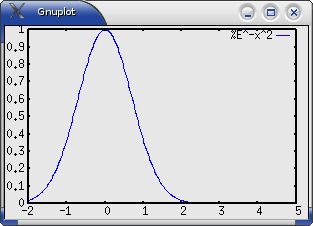
\includegraphics[scale=1.0]{gnuplot1.png} \\
\emph{a)} \\ 
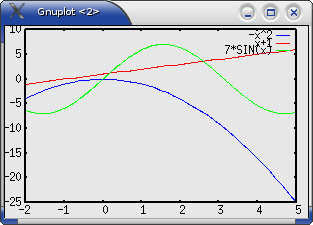
\includegraphics[scale=1.0]{gnuplot2.png} \\
\emph{b)} \\
\caption{Funciones en coordenadas cartesianas: \emph{a)} una sola funci'on; \emph{b)} una familia de funciones.}
\label{fig:gp1}
\end{center}
\end{figure}

Para la realizaci'on de funciones definidas param'etricamente necesitamos hacer uso del s'imbolo \verb|parametric|, Figura~\ref{fig:gp2},
\begin{verbatim}
(%i3) plot2d([parametric,t,t*sin(1/t),[t,0.01,0.2]])$
\end{verbatim}
El resultado que se obtine es el del apartado \emph{a)}. Maxima calcula por defecto un n'umero fijo de puntos de la funci'on que luego utilizar'a para representarla; como esta es una funci'on que var'ia mucho cerca del origen, pediremos que nos haga el dibujo con un mayor n'umero de puntos, lo que se har'a mediante la opci'on \verb|nticks|, tal como se indica a continuaci'on,
\begin{verbatim}
(%i4) plot2d([parametric,t,t*sin(1/t),[t,0.01,0.2],[nticks,500]])$
\end{verbatim}
Se comprueba que el aspecto ha cambiado apreciablemente.

\begin{figure}
\begin{center}
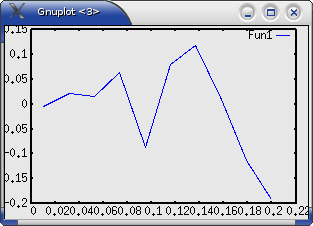
\includegraphics[scale=1.0]{gnuplot3.png} \\
\emph{a)} \\ 
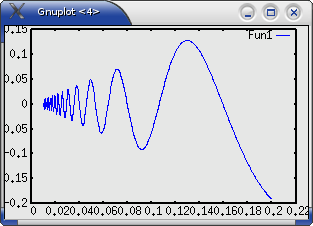
\includegraphics[scale=1.0]{gnuplot4.png} \\
\emph{b)} \\
\caption{Control del n'umero de puntos: \emph{a)} n'umero de puntos por defecto; \emph{b)} la misma funci'on con 500 puntos.}
\label{fig:gp2}
\end{center}
\end{figure}

El siguiente ejemplo muestra la presencia en un mismo gr'afico de la funci'on $y=x^3+2$ junto con la circunferencia de radio unidad, expresada param'etricamente, que en el apartado \emph{a)} de la Figura~\ref{fig:gp3} se ve como una elipse debido a la diferencia de escalas en los ejes,
\begin{verbatim}
(%i5) plot2d([x^3+2,[parametric,cos(t),sin(t),[t,-5,5]]],
(%i6)        [x,-1.3,1.3],[nticks,500])$
\end{verbatim}

Tambi'en es posible la generaci'on de superficies en 3D definidas de la forma $z=f(x,y)$, apartado \emph{b)} de la Figura~\ref{fig:gp3},
\index{plot3d}\begin{verbatim}
(%i7) plot3d(exp(-x^2-y^2),[x,-2,2],[y,-2,0])$
\end{verbatim}

\begin{figure}
\begin{center}
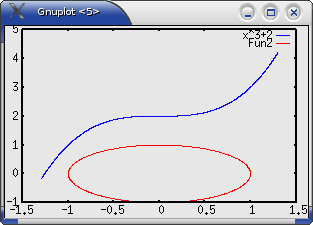
\includegraphics[scale=1.0]{gnuplot5.png} \\
\emph{a)} \\ 
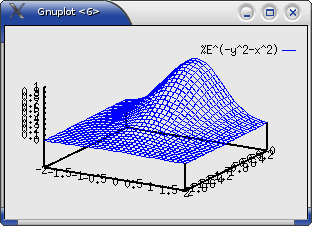
\includegraphics[scale=1.0]{gnuplot6.png} \\
\emph{b)} \\
\caption{M'as tipos de gr'aficos: \emph{a)} combinando funciones param'etrica y no param'etrica; \emph{b)} superficie en 3D.}
\label{fig:gp3}
\end{center}
\end{figure}

Finalmente, del manual de Maxima se ha extra'ido la banda de M\"{o}bius como un ejemplo de superficie param'etica, apartado \emph{a)} de la Figura~\ref{fig:gp4},
\begin{verbatim}
(%i8) plot3d([cos(x)*(3+y*cos(x/2)),
             sin(x)*(3+y*cos(x/2)),y*sin(x/2)],
             [x,-%pi,%pi],[y,-1,1],['grid,50,15]);
\end{verbatim}

La funci'on \verb|plot3d| es capaz de generar una curva param'etrica en tres dimensiones, como lo prueba esta h'elice, que se puede ver en el apartado \emph{b)} de la Figura~\ref{fig:gp4},
\begin{verbatim}
(%i9) plot3d([cos(t),sin(t),2*t],[t,-%pi,%pi],[u,0,1]);
\end{verbatim}

\begin{figure}
\begin{center}
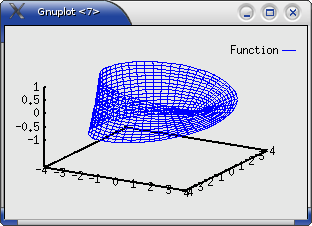
\includegraphics[scale=1.0]{gnuplot7.png} \\
\emph{a)} \\ 
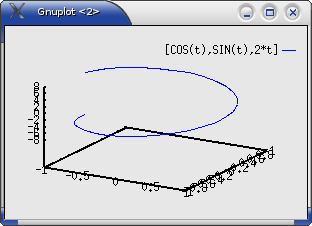
\includegraphics[scale=1.0]{gnuplot8.png} \\
\emph{b)} \\
\caption{Gr'aficos param'etricos en 3D: \emph{a)} una superficie; \emph{b)} una curva.}
\label{fig:gp4}
\end{center}
\end{figure}

El control de las opciones gr'aficas se consigue manipulando la variable global \verb|plot_options|\index{plot\_options}, cuyo estado por defecto es
\begin{verbatim}
(%i10) plot_options;
(%o10) [[x, - 1.755559702014e+305, 1.755559702014e+305], 
[y, - 1.755559702014e+305, 1.755559702014e+305], 
[t, - 3, 3], [GRID, 30, 30], [VIEW_DIRECTION, 1, 1, 1], 
[COLOUR_Z, FALSE], [TRANSFORM_XY, FALSE], 
[RUN_VIEWER, TRUE], [PLOT_FORMAT, GNUPLOT], 
[GNUPLOT_TERM, DEFAULT], [GNUPLOT_OUT_FILE, FALSE], 
[NTICKS, 10], [ADAPT_DEPTH, 10], [GNUPLOT_PM3D, FALSE], 
[GNUPLOT_PREAMBLE, ], [GNUPLOT_CURVE_TITLES, [DEFAULT]], 
[GNUPLOT_CURVE_STYLES, [with lines 3, with lines 1, 
with lines 2, with lines 5, with lines 4, with lines 6, 
with lines 7]], [GNUPLOT_DEFAULT_TERM_COMMAND, ], 
[GNUPLOT_DUMB_TERM_COMMAND, set term dumb 79 22], 
[GNUPLOT_PS_TERM_COMMAND, set size 1.5, 1.5;set term postsc#
ript eps enhanced color solid 24]]
\end{verbatim}
Para mayor informaci'on sobre el significado de cada uno de los elementos de esta lista ser'ia aconsejable ejecutar el comando \verb|describe(plot_options)|.

Ya se ha comentado que a menos que se le indique lo contrario, Maxima invocar'a al programa Gnuplot para la representaci'on de un gr'afico, pero quiz'as prefiramos el programa Openmath, que forma parte de la distribuci'on de Maxima; en tal caso tendr'iamos que modificar previamente las opciones guardadas en \verb|plot_options| y a continuaci'on solicitar el gr'afico deseado, como en este caso en el que se representa la funci'on gamma y su inversa, cuyo resultado se observa en el apartado \emph{a)} de la Figura~\ref{fig:gp5}
\index{set\_plot\_option}\begin{verbatim}
(%i11) set_plot_option([plot_format, openmath])$
(%i12) plot2d([gamma(x),1/gamma(x)],[x,-4.5,5],[y,-10,10])$
\end{verbatim}
Tambi'en Openmath es capaz de realizar gr'aficos en tres dimensiones definidos en coordenadas polares y que se representa en el apartado \emph{b)} de la Figura~\ref{fig:gp5}. N'otese c'omo desde la propia funci'on es posible alterar las opciones gr'aficas; sin embargo, hecho de esta manera los cambios s'olo tienen lugar para la realizaci'on del gr'afico presente, sin alterar las opciones globales.
\begin{verbatim}
(%i13) plot3d(r^0.33*cos(t/3),[r,0,1],[t,0,6*%pi],
              ['grid,20,80],['transform_xy,polar_to_xy])$
\end{verbatim}

\begin{figure}
\begin{center}
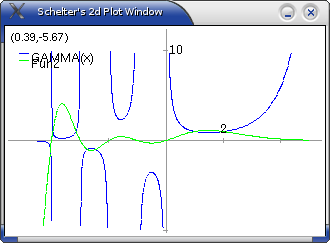
\includegraphics[scale=1.0]{openmath1.png} \\
\emph{a)} \\ 
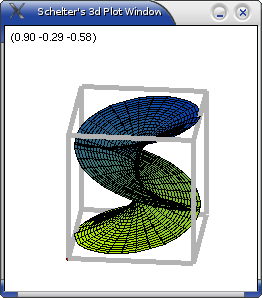
\includegraphics[scale=1.0]{openmath2.png} \\
\emph{b)} \\
\caption{Gr'aficos en Openmath: \emph{a)} en el plano; \emph{b)} en tres dimensiones.}
\label{fig:gp5}
\end{center}
\end{figure}

Las Figuras que se han representado hasta ahora en esta secci'on son capturas de pantalla de la ventana generada por Gnuplot o por Openmath y guardadas en disco en formato PNG. Sin embargo, podemos hacer que el programa gr'afico genere directamente un archivo PNG en lugar de mostrarlo en pantalla. Volvamos a Gnuplot y obtengamos directamente de este programa un archivo con este formato de uno de los gr'aficos que ya realizamos anteriormente,
\index{gnuplot\_preamble}\begin{verbatim}
(%i14) set_plot_option([plot_format, gnuplot])$
(%i15) plot3d(exp(-x^2-y^2),[x,-2,2],[y,-2,0],
              [gnuplot_preamble,"set terminal png size 420,320;
                                 set out 'grafico.png'"])$
\end{verbatim}
Despu'es de cambiar globalmente el programa gr'afico, volvemos a representar la superficie tridimensional que ya vimos en el apartado \emph{b)} de la Figura~\ref{fig:gp3}. V'ease c'omo se ha cambiado el par'ametro gr'afico \verb|gnuplot_preamble| para indicarle a Gnuplot que genere un archivo en formato PNG de ciertas dimensiones dadas y que lo guarde con el nombre \verb|grafico.png|. El resultado lo vemos en el apartado \emph{a)} de la Figura~\ref{fig:gp6}. Cuando se trabaja en Gnuplot, el par'ametro \verb|gnuplot_preamble| permite pasar a este programa una serie de comandos que afinan los detalles; estos comandos deben ir separados por puntos y comas y deben ser los propios del lenguaje de Gnuplot. Para un mejor dominio de estos detalles es aconsejable recurrir a la documentaci'on de este programa (www.gnuplot.info).

Por 'ultimo, si se quiere un archivo gr'afico en Postscript, repitamos el 'ultimo ejemplo solicitando este formato,
\begin{verbatim}
(%i16) plot3d(exp(-x^2-y^2),[x,-2,2],[y,-2,0],
              [gnuplot_preamble,"set terminal postscript eps;
                                 set out 'grafico.eps'"])$
\end{verbatim}
El resultado en el apartado \emph{b)} de la Figura~\ref{fig:gp6}. Los gr'aficos almacenados en formato Postscript, los que tienen extensi'on EPS, suelen ser necesarios cuando se planea crear un documento basado en \TeX-\LaTeX.

\begin{figure}
\begin{center}
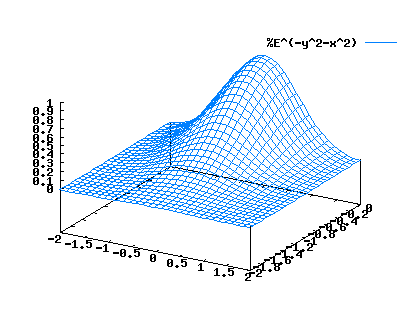
\includegraphics[scale=1.0]{grafico.png} \\
\emph{a)} \\ 
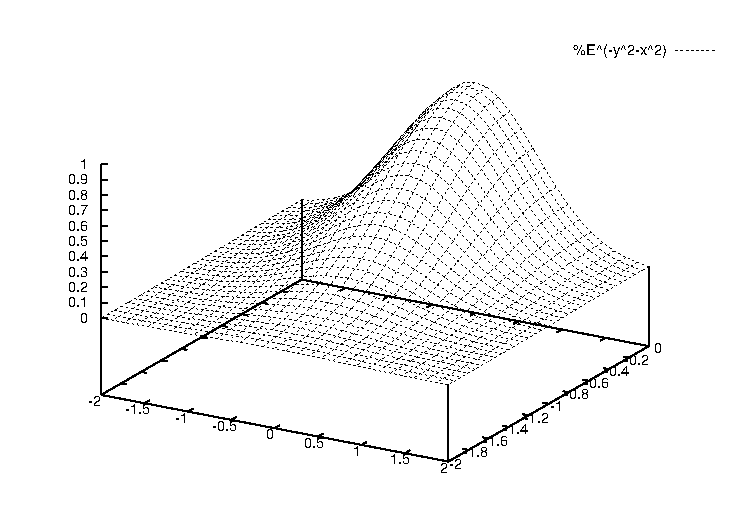
\includegraphics[scale=1.0]{grafico.pdf} \\
\emph{b)} \\
\caption{Formatos de archivos gr'aficos: \emph{a)} PNG; \emph{b)} Postscript.}
\label{fig:gp6}
\end{center}
\end{figure}

Puesto que estamos hablando de \LaTeX, este es un buen lugar para hacer referencia a una funci'on que transforma una expresi'on de Maxima a formato \TeX, de manera que el resultado que se obtenga pueda ser incorporado f'acilmente (copiar y pegar) a un archivo fuente de \LaTeX; a modo de ejemplo, calculemos una derivada para posteriormente transformarla,
\index{4@'}\index{tex}\begin{verbatim}
(%i17) 'diff(sin(x^x)*sqrt(log(x)),x)=
           diff(sin(x^x)*sqrt(log(x)),x);
       d                     x
(%o17) -- (sqrt(log(x)) sin(x )) =
       dx

              x
         sin(x )         x                                x
     ---------------- + x  sqrt(log(x)) (log(x) + 1) cos(x )
     2 x sqrt(log(x))
(%i18) tex(%);

$${{d}\over{d\,x}}\,\left(\sqrt{\log x}\,\sin x^{x}\right)={{\sin x^{
 x}}\over{2\,x\,\sqrt{\log x}}}+x^{x}\,\sqrt{\log x}\,\left(\log x+1
 \right)\,\cos x^{x}$$
(%o18)                      false
\end{verbatim}
El ap'ostrofo que se coloca en la entrada \verb|(%i17)| antes de la funci'on \verb|diff| sirve para devolver la expresi'on sin evaluarla, tal como aparece en el miembro izquierdo de la igualdad \verb|(%o17)|. Una vez copiada y pegada la respuesta de la entrada \verb|(%i18)| en una fuente \LaTeX, su compilaci'on dar'a como resultado la expresi'on
\[
{{d}\over{d\,x}}\,\left(\sqrt{\log x}\,\sin x^{x}\right)={{\sin x^{
 x}}\over{2\,x\,\sqrt{\log x}}}+x^{x}\,\sqrt{\log x}\,\left(\log x+1
 \right)\,\cos x^{x}
\]
m'as f'acil de interpretar por un humano.


\newpage
\section{Listas}

Las listas son objetos muy potentes a la hora de representar estructuras de datos; de hecho, toda expresi'on de Maxima se representa internamente como una lista, lo que no es de extra~nar habida cuenta de que Maxima est'a programado en Lisp (\emph{List Processing}). Veamos c'omo podemos ver la representaci'on interna, esto es en Lisp, de una sencilla expresi'on tal como $1+3a$,
\index{31@:lisp}\begin{verbatim}
(%i1) :lisp #$1+3*a$
((MPLUS SIMP) 1 ((MTIMES SIMP) 3 $a))
\end{verbatim}
N'otese que el formato general es de la forma \verb|:lisp #$expr$|, siendo \verb|expr| una expresi'on cualquiera en Maxima.

Pero al nivel del usuario que no est'a interesado en las interioridades de Maxima, tambi'en se puede trabajar con listas como las definidas a continuaci'on, simpre encerradas entre corchetes,
\index{34@[...]}\index{32@``...''}\begin{verbatim}
(%i2) q:[b,5,a,d,1,3,7]$
(%i3) r:[1,[a,3],sqrt(3)/2,"Don Quijote"];
                         sqrt(3)
(%o3)        [1, [a, 3], -------, Don Quijote]
                            2
\end{verbatim}
Vemos que los elementos de una lista pueden a su vez ser tambi'en listas, expresiones matem'aticas o cadenas de caracteres incluidas entre comillas dobles, lo que puede ser aprovechado para la construcci'on y manipulaci'on de estructuras m'as o menos complejas. Extraigamos a continuaci'on alguna informaci'on de las listas anteriores,
\index{listp}\index{first}\index{second}\index{third}\index{last}\index{rest}\index{part}\index{length}\index{reverse}\index{member}\index{sort}\index{delete}\begin{verbatim}
(%i4) listp(r); /* es r una lista? */
(%o4)                       true
(%i5) first(r); /* primer elemento */
(%o5)                        1
(%i6) second(r); /* segundo elemento */
(%o6)                      [a, 3]
(%i7) third(r); /* ...hasta tenth */
                          sqrt(3)
(%o7)                     -------
                             2
(%i8) last(r); /* el ultimo de la lista */
(%o8)                   Don Quijote
(%i9) rest(r); /* todos menos el primero */
                        sqrt(3)
(%o9)         [[a, 3], -------, Don Quijote]
                           2
(%i10) part(r,3); /* pido el que quiero */
                          sqrt(3)
(%o10)                    -------
                             2
(%i11) length(r); /* cuantos hay? */
(%o11)                       4
(%i12) reverse(r); /* le damos la vuelta */
                           sqrt(3)
(%o12)       [Don Quijote, -------, [a, 3], 1]
                              2
(%i13) member(a,r); /* es a un elemento?*/
(%o13)                     false
(%i14) member([a,3],r); /* lo es [a,3]? */
(%o14)                      true
(%i15) sort(q); /* ordeno */
(%o15)             [1, 3, 5, 7, a, b, d]
(%i16) delete([a,3],r); /* borro elemento */
                     sqrt(3)
(%o16)           [1, -------, Don Quijote]
                        2
\end{verbatim}
N'otese que en todo este tiempo la lista \verb|r| no se ha visto alterada,
\begin{verbatim}
(%i17) r;
                         sqrt(3)
(%o18)       [1, [a, 3], -------, Don Quijote]
                            2
\end{verbatim}

Algunas funciones de Maxima permiten a~nadir nuevos elementos a una lista, tanto al principio como al final,
\index{cons}\index{endcons}\begin{verbatim}
(%i19) cons(1+2,q);
(%o19)            [3, b, 5, a, d, 1, 3, 7]
(%i20) endcons(x,q);
(%o20)            [b, 5, a, d, 1, 3, 7, x]
\end{verbatim}
En este ejemplo observamos tambi'en que la lista \verb|q| no ha cambiado; si lo que queremos es actualizar su contenido,
\begin{verbatim}
(%i26) q: endcons(x,cons(1+2,q))$
(%i27) q;
(%o27)          [3, b, 5, a, d, 1, 3, 7, x]
\end{verbatim}

Es posible unir dos listas,
\index{append}\begin{verbatim}
(%i28) append(r,q);
                   sqrt(3)
(%o28) [1, [a, 3], -------, Don Quijote, 3, b, 5, a, d, 1,
                      2

                                                    3, 7, x]
\end{verbatim}

Cuando los elementos de una lista van a obedecer un cierto criterio de construcci'on, podemos utilizar la funci'on \verb|makelist|\index{makelist},
\begin{verbatim}
(%i29) s:makelist(2+k*2,k,0,10);
(%o29)    [2, 4, 6, 8, 10, 12, 14, 16, 18, 20, 22]
\end{verbatim}
donde le hemos indicado a Maxima que nos construya una lista con elementos de la forma \verb|2+2*k|, de modo que \verb|k| tome valores enteros de 0 a 10.

La funci'on \verb|apply|\index{apply} permite suministrar a otra funci'on todos los elementos de una lista como argumentos, as'i podemos sumar o multiplicar todos los elementos de la lista \verb|s| reci'en creada,
\index{14@+}\index{16@*}\begin{verbatim}
(%i30) apply("+",s);
(%o30)                      132
(%i31) apply("*",s);
(%o31)                  81749606400
\end{verbatim}
aunque estas dos operaciones hubiese sido quiz'as mejor haberlas realizado con las funciones \verb|sum|\index{sum} y \verb|product|\index{product}.

A veces interesar'a aplicar una misma funci'on a varios elementos de una lista de forma independiente, para lo que haremos uso de \verb|map|\index{map}; a continuaci'on un ejemplo de c'alculo de factoriales y otro trigonom'etrico,
\begin{verbatim}
(%i32) map("!",s);
(%o32) [2, 24, 720, 40320, 3628800, 479001600, 87178291200,
20922789888000, 6402373705728000, 2432902008176640000,
1124000727777607680000]
(%i33) map(sin,s);
(%o33) [sin(2), sin(4), sin(6), sin(8), sin(10), sin(12),
                sin(14), sin(16), sin(18), sin(20), sin(22)]
\end{verbatim}

Por 'ultimo, las listas tambi'en pueden ser utilizadas en operaciones aritm'eticas,
\index{14@+}\index{15@-}\index{16@*}\index{17@/}\index{18@\^\ }\index{21@.}\begin{verbatim}
(%i34) [1,2,3]+[a,b,c];
(%o34)             [a + 1, b + 2, c + 3]
(%i35) [1,2,3]*[a,b,c];
(%o35)                 [a, 2 b, 3 c]
(%i36) [1,2,3]/[a,b,c];
                          1  2  3
(%o36)                   [-, -, -]
                          a  b  c
(%i37) [1,2,3]-[a,b,c];
(%o37)             [1 - a, 2 - b, 3 - c]
(%i38) [1,2,3].[a,b,c]; /* producto escalar */
(%o38)                 3 c + 2 b + a
(%i39) [a,b,c]^3;
                          3   3   3
(%o39)                  [a , b , c ]
(%i40) 3^[a,b,c];
                          a   b   c
(%o40)                  [3 , 3 , 3 ]
\end{verbatim}
Para que estas operaciones puedan realizarse sin problemas, la variable global \verb|listarith|\index{listarith} debe tomar el valor \verb|true|, en caso contrario el resultado ser'a bien distinto,
\begin{verbatim}
(%i41) listarith:false$
(%i42) [1,2,3]+[4,5,6];
(%o42)             [4, 5, 6] + [1, 2, 3]
(%i43) listarith:true$
\end{verbatim}

Como ya se vi'o al comienzo de esta secci'on, una lista puede ser elemento de otra lista, si queremos deshacer todas las listas interiores para que sus elementos pasen a formar parte de la exterior,
\index{flatten}\begin{verbatim}
(%i44) flatten([1,[a,b],2,3,[c,[d,e]]]);
(%o44)            [1, a, b, 2, 3, c, d, e]
\end{verbatim}


\newpage
\section{Operaciones con conjuntos}

Se define a continuaci'on un conjunto mediante la funci'on \verb|set|\index{set},
\begin{verbatim}
(%i1) c1:set(a,[2,k],b,sqrt(2),a,set(a,b),
             3,"Sancho",set(),b,sqrt(2),a);
(%o1)  {3, sqrt(2), {}, [2, k], a, {a, b}, b, Sancho}
\end{verbatim}
Como se ve, se admiten objetos de muy diversa naturaleza como elementos de un conjunto: n'umeros, expresiones, el conjunto vac'io (\verb|{}|), listas, otros conjuntos o cadenas de caracteres. Cuando se trabaja con listas, puede ser de utilidad considerar sus componentes como elementos de un conjunto, luego se necesita una funci'on que nos transforme una lista en conjunto,
\index{setify}\begin{verbatim}
(%i2) [[2,k],sqrt(2),set(b,a),[k,2],"Panza"];
(%o2)     [[2, k], sqrt(2), {a, b}, [k, 2], Panza]
(%i3) c2:setify(%);
(%o3)     {sqrt(2), [2, k], {a, b}, [k, 2], Panza}
\end{verbatim}
el cambio en la naturaleza de estas dos colecciones de objetos se aprecia en la presencia de llaves frente a los corchetes. De igual manera, podemos transformar un conjunto en lista,
\index{listify}\begin{verbatim}
(%i4) listify(%o1);
(%o4)  [3, sqrt(2), {}, [2, k], a, {a, b}, b, Sancho]
\end{verbatim}
Comprobemos de paso que \verb|{}| representa al conjunto vac'io,
\index{emptyp}\begin{verbatim}
(%i5) emptyp(%[3]);
(%o5)                      true
\end{verbatim}
Recu'erdese que \verb|%| sustituye a la 'ultima respuesta dada por Maxima, que en este caso hab'ia sido una lista, por lo que \verb|%[3]| hace referencia a su tercera componente.

Para comprobar si un cierto objeto forma parte de un conjunto hacemos uso de la instrucci'on \verb|elementp|\index{elementp},
\begin{verbatim}
(%i6) elementp(sqrt(2),c1);
(%o6)                      true
\end{verbatim}
Es posible extraer un elemento de un conjunto y luego a~nadirle otro distinto
\index{disjoin}\index{adjoion}\begin{verbatim}
(%i7) c1: disjoin(sqrt(2),c1);  /* sqrt(2) fuera */
(%o7)     {3, {}, [2, k], a, {a, b}, b, Sancho}
(%i8) c1: adjoin(sqrt(3),c1);  /* sqrt(3) dentro */
(%o8) {3, sqrt(3), {}, [2, k], a, {a, b}, b, Sancho}
\end{verbatim}
La sustituci'on que se acaba de realizar se pudo haber hecho con la funci'on \verb|subst|\index{subst},
\begin{verbatim}
(%i9) /* nuevamente a poner sqrt(2) */
      subst(sqrt(2),sqrt(3),c1);
(%o9) {3, sqrt(2), {}, [2, k], a, {a, b}, b, Sancho}
\end{verbatim}

La comprobaci'on de si un conjunto es subconjunto de otro se hace con la fuci'on \verb|subsetp|\index{subsetp},
\begin{verbatim}
(%i10) subsetp(set([k,2],"Panza"),c2);
(%o10)                      true
\end{verbatim}

A continuaci'on algunos ejemplos de operaciones con conjuntos,
\index{union}\index{intersection}\index{setdifference}\index{cardinality}\begin{verbatim}
(%i11) union(c1,c2);
(%o11) {3, sqrt(2), sqrt(3), {}, [2, k], a, {a, b}, b,
                                      [k, 2], Panza, Sancho}
(%i12) intersection(c1,c2);
(%o12)                {[2, k], {a, b}}
(%i13) setdifference(c1,c2);
(%o13)         {3, sqrt(3), {}, a, b, Sancho}
(%i14) cardinality(%);
(%o14)                       6
\end{verbatim}
Vemos aqu'i tambi'en c'omo pedir el cardinal de un conjunto.

Igual que se ha visto como aplicar una funci'on a todos los elementos de una lista, podemos hacer lo mismo con los de un conjunto,
\index{map}\begin{verbatim}
(%i15) map(sin,set(1,2,3,4,5));
(%o15)    {sin(1), sin(2), sin(3), sin(4), sin(5)}
\end{verbatim}

Por 'ultimo ya, el producto cartesiano de tres conjuntos,
\index{cartesianproduct@cartesian\_product}\begin{verbatim}
(%i16) cartesian_product(set(1,2),set(a,b,c),set(x,y));
(%o16) {[1, a, x], [1, a, y], [1, b, x], [1, b, y],
[1, c, x], [1, c, y], [2, a, x], [2, a, y], [2, b, x],
[2, b, y], [2, c, x], [2, c, y]}
\end{verbatim}

\newpage
\section{Operaciones l'ogicas}

Como cualquier otro int'erprete o entorno de programaci'on, Maxima dispone tambi'en de la capacidad de evaluar predicados l'ogicos, aqu'ellos que pueden ser o bien verdaderos (\verb|true|)\index{true}, o bien falsos (\verb|false|)\index{false}. Los predicados m'as simples son funciones que devuelven uno de estos dos valores de verdad; ejemplos de ellos ya han aparecido en secciones anteriores,
\begin{verbatim}
(%i1) listp([[1,2],[a,b]]);
(%o1)                       true
(%i2) matrixp([[1,2],[a,b]]);
(%o2)                      false
(%i3) evenp(2^3);
(%o3)                       true
\end{verbatim}

Puesto que Maxima es un entorno de procesamiento matem'atico, es frecuente tener que comparar dos cantidades. Los operadores de comparaci'on se resumen en la siguiente tabla,
\index{22@=}\index{23@\#}\index{24@$>$}\index{25@$<$}\index{26@$>=$}\index{27@$=<$}\begin{center}
\begin{tabular}{|c|c|} \hline
\verb|=|  &  ...igual que...         \\ \hline
\verb|#| &  ...diferente de...     \\ \hline
\verb|>|  &  ...mayor que...         \\ \hline
\verb|<|  &  ...menor que...         \\ \hline
\verb|>=| &  ...mayor o igual que... \\ \hline
\verb|=<| &  ...menor o igual que... \\ \hline
\end{tabular}
\end{center}

Si se quiere saber si un n'umero es menor que otro podemos hacer uso de la funci'on \verb|is|\index{is},
\begin{verbatim}
(%i4) is(sqrt(7895)<85);
(%o4)                      false
(%i5) is(4^12#16777216);
(%o5)                      false
\end{verbatim}
En el primer caso comprobamos si $\sqrt{7895}$ es estrictamente menor que 85 y en el segundo si la potencia $4^{12}$ es diferente de 16777216.

Junto con estos predicados simples, los conectores \verb|and|\index{and}, \verb|or|\index{or} y \verb|not|\index{not} permiten construir formas m'as complejas. La tabla adjunta resume el comportamiento de estos operadores,
\begin{center}
\begin{tabular}{|c|c||c|c|c|} \hline
     p       &       q      & p \verb|and| q & p \verb|or| q & \verb|not| p  \\ \hline
\verb|false| & \verb|false| & \verb|false|   & \verb|false|  & \verb|true|  \\
\verb|false| & \verb|true|  & \verb|false|   & \verb|true|   & \verb|true|  \\
\verb|true|  & \verb|false| & \verb|false|   & \verb|true|   & \verb|false|  \\
\verb|true|  & \verb|true|  & \verb|true|    & \verb|true|   & \verb|false|  \\ \hline
\end{tabular}
\end{center}

A la hora de escribir expresiones l'ogicas conviene tener en cuenta el orden de precedencia; primero se eval'ua \verb|not|, a continuaci'on \verb|and| y, finalmente, \verb|or|; en caso de duda siempre se puede recurrir a los par'entesis. Un ejemplo,
\begin{verbatim}
(%i6) is(not 3<4 or 5<5);
(%o6)                      false
\end{verbatim}
Aqu'i, primero se eval'ua \verb|not 3<4|, que da como resultado \verb|false|; a continuaci'on, se eval'ua si es cierto o no que \verb|5<5|, lo cual es tambi'en falso, finalmente se obtiene el resultado correspondiente a \verb|false or false|.

El lector deber'ia ser capaz de justificar las siguientes respuestas,
\begin{verbatim}
(%i7) is(3#4 and not 7<=2);
(%o7)                       true
(%i8) is((5<8 or 8<2) and oddp(3) and evenp(sqrt(16)));
(%o8)                       true
\end{verbatim}


\newpage
\section{Programaci'on en Maxima}

Con vistas a la optimizaci'on de tiempo y esfuerzo ser'a interesante poder definir de una sola vez nuestras propias funciones y poder luego reutilizarlas cuantas veces sea necesario.

La programaci'on de funciones requiere de ciertas sentencias de control que son comunes, con m'as o menos matices en su sintaxis, en todos los lenguajes de programaci'on.

Un elemento imprescindible en el control del flujo es la sentencia condicional \verb|if|\index{if-then-else}, cuya estructura es
\begin{verbatim}
          if <cond> then <expr1> else <expr2>
\end{verbatim}
tal como en
\begin{verbatim}
(%i1) x:30!$ y:exp(30)$
(%i3) if (x>y) then 0 else 1;
(%o3)                       0
\end{verbatim}

La condici'on \verb|<cond>| es una expresi'on l'ogica que admite los operadores \verb|and|\index{and}, \verb|or|\index{or} y \verb|not|\index{not}, siendo sus argumentos predicados l'ogicos, cuyo valor s'olo puede ser \emph{verdadero} o \emph{falso},

Otra sentencia que nunca falta en un lenguaje de programaci'on es la que controla las iteraciones y los bucles. Maxima ofrece aqu'i varias posibilidades. En primer lugar,
\index{for}\begin{verbatim}
      for <var>:<val1> step <val2> thru <val3> do <expr>
\end{verbatim}
El siguiente ejemplo escribe, haciendo uso de la funci'on \verb|print|\index{print}, los cinco primeros cubos enteros positivos,
\begin{verbatim}
(%i4) for i:1 thru 5 do print(i^3);
1
8
27
64
125
(%o4)                      done
\end{verbatim}

Otra posibilidad de controlar las iteraciones es con la versi'on
\begin{verbatim}
      for <var>:<val1> step <val2> while <cond> do <expr>
\end{verbatim}
que en el siguiente ejemplo se utiliza para calcular las quintas potencias de todos los n'umeros impares menores que 20; n'otese c'omo tras la sentencia \verb|do| se pueden escribir varias expresiones separadas por comas (\verb|,|)\index{2@, (coma)} y encerradas entre par'entesis,
\begin{verbatim}
(%i5) for i:1 step 2 while i<20 do(j:i^5,print(j));
1
243
3125
16807
59049
161051
371293
759375
1419857
2476099
(%o5)                      done
\end{verbatim}

Tambi'en hay una versi'on de la sentencia \verb|for| muy a prop'osito para trabajar con listas,
\begin{verbatim}
          for <var> in <lista> do <expr>
\end{verbatim}
como se muestra en el siguiente ejemplo, donde se imprimen todos los elementos de una muestra simulada de n'umeros aleatorios, aumentados en una unidad,
\begin{verbatim}
(%i7) m:makelist(random(4),i,1,10);
(%o7)         [2, 0, 3, 2, 2, 3, 0, 1, 1, 3]
(%i8) for i in m do print(i+1);
3
1
4
3
3
4
1
2
2
4
(%o8)                      done
\end{verbatim}

En general, la definici'on de una nueva funci'on en Maxima tiene la estructura
\begin{verbatim}
          f(<arg1>,<arg2>,...):=<expr>
\end{verbatim}
donde \verb|<argi>| son los argumentos y \verb|<expr>| es una expresi'on sint'acticamente v'alida. Por ejemplo, ya que Maxima no dispone de la funci'on logaritmo en base arbitraria, la podemos definir por nuestra cuenta,
\index{28@:=}\begin{verbatim}
(%i9) logb(x,b):=log(x)/log(b)$
(%i10) logb(234,10);
                          log(234)
(%o10)                    --------
                          log(10)
(%i11) %,numer;
(%o11)                    2.3692157
\end{verbatim}

En ocasiones, la funci'on es lo suficientemente compleja como para necesitar tanto de variables locales que guarden valores temporales, como de expresiones que los calculen; en tales casos habr'a que echar mano del entorno de boque con la instrucci'on \verb|block|\index{block}, cuya estructura es
\begin{verbatim}
          f(<arg1>,<arg2>,...):=block([<varloc1>,<varloc2>,...],
             <expr1>,
             <expr2>,
               ....
             <exprm> );
\end{verbatim}
siendo el resultado devuelto el de la 'ultima expresi'on evaluada (\verb|<exprm>|). Las variables locales a las que se ha hecho referencia se declaran entre corchetes (\verb|<varloci>|) dentro del bloque, donde pueden ser inicializadas y cuya vida se extiende durante el tiempo que dure el c'omputo del bloque; adem'as, si una de estas variables temporales se llama igual que otra global de la sesi'on de Maxima, no interferir'a con ella y cualquier referencia a la variable se considerar'a que es a la local, y en caso de que 'esta no est'e declarada, la referencia ser'a a la externa a la funci'on. A continuaci'on, un ejemplo en el que se define una funci'on que calcula la media de una lista de n'umeros,
\begin{verbatim}
(%i12) media(lista):=block([n:length(lista),suma],
   if not listp(lista)
      then return("Ojo: no es una lista"),
   suma: sum(lista[k],k,1,n),
   suma/n )$
(%i13) media([45,25,87,23,65,31]);
(%o13)                       46
(%i14) media([[2,3],[6,3],[4,7],[2,6]]);
                           7  19
(%o14)                    [-, --]
                           2  4
(%i15) media([1/3,sqrt(5),logb(5,2),x]);
                      log(5)             1
                  x + ------ + sqrt(5) + -
                      log(2)             3
(%o15)            ------------------------
                             4
(%i16) solve(%=10,x);  /* cuanto vale x para una media de 10? */
               3 log(5) + (3 sqrt(5) - 119) log(2)
(%o16)  [x = - -----------------------------------]
                            3 log(2)
\end{verbatim}
Este 'ultimo c'alculo no tiene nada que ver con lo que se comenta en esta secci'on, pero muestra c'omo integrar nuestra funci'on en una sesi'on rutinaria. Examinando el c'odigo de la funci'on \verb|media| reparamos en la presencia de la instrucci'on \verb|return|, que es una forma alternativa de salir del contexto marcado por \verb|block|; en este caso, el resultado que devuelve la funci'on es el indicado por el argumento de \verb|return|\index{return}, es decir la cadena \verb|"Ojo: no es una lista"|. Tambi'en se observa que se declaran dos variables locales, \verb|n| y \verb|suma|, asign'andole a la primera el n'umero de elementos de la lista; junto con 'estas existe otra variable local, la \verb|k| de la instrucci'on \verb|sum|, que s'olo est'a activa durante el c'alculo de esta suma, no siendo necesario declararla en todo el contexto del bloque.

A veces es necesario definir funciones cuyo n'umero de argumentos no se conoce a priori. Por ejemplo, tal como est'a programada la funci'on \verb|gcd|\index{gcd} en Maxima, la que calcula el m'aximo com'un divisor, no admite m'as de dos argumentos; podemos suplir esta carencia dise~nando una funci'on, que llamaremos \verb|mcd|, y que admita un n'umero arbitrario de n'umeros,
\begin{verbatim}
(%i17) mcd(a,b,[c]):=block([n],
   n: length(c),
   r: gcd(a,b),
   if n>0 then
      for i in c do r: gcd(r,i),
   r )$
(%i18) mcd(120,300,480,825);
(%o18)                       15
\end{verbatim}

Por 'ultimo ya, se a~nade un ejemplo en el que se define una funci'on haciendo uso de algunas de las sentencias comentadas en esta secci'on. Como se ve, a la funci'on se le asigna el nombre de \verb|transafin| y su cometido es el de aplicar una transformaci'on af'in a una lista de puntos,
\begin{verbatim}
/*Asi se escriben los comentarios. */
/*pts debe ser una lista de pares: */
/* [[x1,y1],[x2,y2],[x3,y3],...]   */
transafin(pts, a, b, c, d, e, f):=
  block([pts2, n, i, x, y],
    pts2: copylist(pts),
    n: length(pts2),
    for i:1 thru n do(
      x: pts2[i][1],
      y: pts2[i][2],
      pts2[i][1]: a*x+b*y+c,
      pts2[i][2]: d*x+e*y+f ),
    return(pts2) )$
\end{verbatim}

La funci'on \verb|transafin|, y cualquier otra dentro de esta secci'on, se puede escribir en Maxima y luego llamarla para que realice su cometido; sin embargo, quiz'as sea mejor escribirla directamente con un editor de texto cualquiera y guardarla en un archivo, pongamos de nombre \verb|tf.mac|, para hacer uso de ella en el futuro; as'i, una vez dentro de Maxima ejecutar'iamos la instrucci'on \verb|batch("tf.mac")| y luego har'iamos
\begin{verbatim}
(%i19) cuadrado:[[0,0],[1,0],[1,1],[0,1]]$
(%i20) transafin(cuadrado,-1,0,-1,0,1,1);
(%o20)      [[- 1, 1], [- 2, 1], [- 2, 2], [- 1, 2]]
\end{verbatim}
obteniendo as'i el resultado de aplicarle a los v'ertices del cuadrado unidad una simetr'ia respecto del eje de ordenadas seguida de una traslaci'on a lo largo del vector $\vec{v}=(-1,1)$.

\newpage
\section{GNU Free Documentation License}


\tiny

 \begin{center}

       Version 1.2, November 2002


 Copyright \copyright 2000,2001,2002  Free Software Foundation, Inc.
 
 \bigskip
 
     59 Temple Place, Suite 330, Boston, MA  02111-1307  USA
  
 \bigskip
 
 Everyone is permitted to copy and distribute verbatim copies
 of this license document, but changing it is not allowed.
\end{center}


\begin{center}
{\bf Preamble}
\end{center}

The purpose of this License is to make a manual, textbook, or other
functional and useful document "free" in the sense of freedom: to
assure everyone the effective freedom to copy and redistribute it,
with or without modifying it, either commercially or noncommercially.
Secondarily, this License preserves for the author and publisher a way
to get credit for their work, while not being considered responsible
for modifications made by others.

This License is a kind of "copyleft", which means that derivative
works of the document must themselves be free in the same sense.  It
complements the GNU General Public License, which is a copyleft
license designed for free software.

We have designed this License in order to use it for manuals for free
software, because free software needs free documentation: a free
program should come with manuals providing the same freedoms that the
software does.  But this License is not limited to software manuals;
it can be used for any textual work, regardless of subject matter or
whether it is published as a printed book.  We recommend this License
principally for works whose purpose is instruction or reference.


\begin{center}
{\bf 1. APPLICABILITY AND DEFINITIONS}
\end{center}

This License applies to any manual or other work, in any medium, that
contains a notice placed by the copyright holder saying it can be
distributed under the terms of this License.  Such a notice grants a
world-wide, royalty-free license, unlimited in duration, to use that
work under the conditions stated herein.  The \textbf{"Document"}, below,
refers to any such manual or work.  Any member of the public is a
licensee, and is addressed as \textbf{"you"}.  You accept the license if you
copy, modify or distribute the work in a way requiring permission
under copyright law.

A \textbf{"Modified Version"} of the Document means any work containing the
Document or a portion of it, either copied verbatim, or with
modifications and/or translated into another language.

A \textbf{"Secondary Section"} is a named appendix or a front-matter section of
the Document that deals exclusively with the relationship of the
publishers or authors of the Document to the Document's overall subject
(or to related matters) and contains nothing that could fall directly
within that overall subject.  (Thus, if the Document is in part a
textbook of mathematics, a Secondary Section may not explain any
mathematics.)  The relationship could be a matter of historical
connection with the subject or with related matters, or of legal,
commercial, philosophical, ethical or political position regarding
them.

The \textbf{"Invariant Sections"} are certain Secondary Sections whose titles
are designated, as being those of Invariant Sections, in the notice
that says that the Document is released under this License.  If a
section does not fit the above definition of Secondary then it is not
allowed to be designated as Invariant.  The Document may contain zero
Invariant Sections.  If the Document does not identify any Invariant
Sections then there are none.

The \textbf{"Cover Texts"} are certain short passages of text that are listed,
as Front-Cover Texts or Back-Cover Texts, in the notice that says that
the Document is released under this License.  A Front-Cover Text may
be at most 5 words, and a Back-Cover Text may be at most 25 words.

A \textbf{"Transparent"} copy of the Document means a machine-readable copy,
represented in a format whose specification is available to the
general public, that is suitable for revising the document
straightforwardly with generic text editors or (for images composed of
pixels) generic paint programs or (for drawings) some widely available
drawing editor, and that is suitable for input to text formatters or
for automatic translation to a variety of formats suitable for input
to text formatters.  A copy made in an otherwise Transparent file
format whose markup, or absence of markup, has been arranged to thwart
or discourage subsequent modification by readers is not Transparent.
An image format is not Transparent if used for any substantial amount
of text.  A copy that is not "Transparent" is called \textbf{"Opaque"}.

Examples of suitable formats for Transparent copies include plain
ASCII without markup, Texinfo input format, LaTeX input format, SGML
or XML using a publicly available DTD, and standard-conforming simple
HTML, PostScript or PDF designed for human modification.  Examples of
transparent image formats include PNG, XCF and JPG.  Opaque formats
include proprietary formats that can be read and edited only by
proprietary word processors, SGML or XML for which the DTD and/or
processing tools are not generally available, and the
machine-generated HTML, PostScript or PDF produced by some word
processors for output purposes only.

The \textbf{"Title Page"} means, for a printed book, the title page itself,
plus such following pages as are needed to hold, legibly, the material
this License requires to appear in the title page.  For works in
formats which do not have any title page as such, "Title Page" means
the text near the most prominent appearance of the work's title,
preceding the beginning of the body of the text.

A section \textbf{"Entitled XYZ"} means a named subunit of the Document whose
title either is precisely XYZ or contains XYZ in parentheses following
text that translates XYZ in another language.  (Here XYZ stands for a
specific section name mentioned below, such as \textbf{"Acknowledgements"},
\textbf{"Dedications"}, \textbf{"Endorsements"}, or \textbf{"History"}.)  
To \textbf{"Preserve the Title"}
of such a section when you modify the Document means that it remains a
section "Entitled XYZ" according to this definition.

The Document may include Warranty Disclaimers next to the notice which
states that this License applies to the Document.  These Warranty
Disclaimers are considered to be included by reference in this
License, but only as regards disclaiming warranties: any other
implication that these Warranty Disclaimers may have is void and has
no effect on the meaning of this License.


\begin{center}
{\bf 2. VERBATIM COPYING}
\end{center}

You may copy and distribute the Document in any medium, either
commercially or noncommercially, provided that this License, the
copyright notices, and the license notice saying this License applies
to the Document are reproduced in all copies, and that you add no other
conditions whatsoever to those of this License.  You may not use
technical measures to obstruct or control the reading or further
copying of the copies you make or distribute.  However, you may accept
compensation in exchange for copies.  If you distribute a large enough
number of copies you must also follow the conditions in section 3.

You may also lend copies, under the same conditions stated above, and
you may publicly display copies.


\begin{center}
{\bf 3. COPYING IN QUANTITY}
\end{center}


If you publish printed copies (or copies in media that commonly have
printed covers) of the Document, numbering more than 100, and the
Document's license notice requires Cover Texts, you must enclose the
copies in covers that carry, clearly and legibly, all these Cover
Texts: Front-Cover Texts on the front cover, and Back-Cover Texts on
the back cover.  Both covers must also clearly and legibly identify
you as the publisher of these copies.  The front cover must present
the full title with all words of the title equally prominent and
visible.  You may add other material on the covers in addition.
Copying with changes limited to the covers, as long as they preserve
the title of the Document and satisfy these conditions, can be treated
as verbatim copying in other respects.

If the required texts for either cover are too voluminous to fit
legibly, you should put the first ones listed (as many as fit
reasonably) on the actual cover, and continue the rest onto adjacent
pages.

If you publish or distribute Opaque copies of the Document numbering
more than 100, you must either include a machine-readable Transparent
copy along with each Opaque copy, or state in or with each Opaque copy
a computer-network location from which the general network-using
public has access to download using public-standard network protocols
a complete Transparent copy of the Document, free of added material.
If you use the latter option, you must take reasonably prudent steps,
when you begin distribution of Opaque copies in quantity, to ensure
that this Transparent copy will remain thus accessible at the stated
location until at least one year after the last time you distribute an
Opaque copy (directly or through your agents or retailers) of that
edition to the public.

It is requested, but not required, that you contact the authors of the
Document well before redistributing any large number of copies, to give
them a chance to provide you with an updated version of the Document.


\begin{center}
{\bf 4. MODIFICATIONS}
\end{center}

You may copy and distribute a Modified Version of the Document under
the conditions of sections 2 and 3 above, provided that you release
the Modified Version under precisely this License, with the Modified
Version filling the role of the Document, thus licensing distribution
and modification of the Modified Version to whoever possesses a copy
of it.  In addition, you must do these things in the Modified Version:

\begin{itemize}
\item[A.] 
   Use in the Title Page (and on the covers, if any) a title distinct
   from that of the Document, and from those of previous versions
   (which should, if there were any, be listed in the History section
   of the Document).  You may use the same title as a previous version
   if the original publisher of that version gives permission.
   
\item[B.]
   List on the Title Page, as authors, one or more persons or entities
   responsible for authorship of the modifications in the Modified
   Version, together with at least five of the principal authors of the
   Document (all of its principal authors, if it has fewer than five),
   unless they release you from this requirement.
   
\item[C.]
   State on the Title page the name of the publisher of the
   Modified Version, as the publisher.
   
\item[D.]
   Preserve all the copyright notices of the Document.
   
\item[E.]
   Add an appropriate copyright notice for your modifications
   adjacent to the other copyright notices.
   
\item[F.]
   Include, immediately after the copyright notices, a license notice
   giving the public permission to use the Modified Version under the
   terms of this License, in the form shown in the Addendum below.
   
\item[G.]
   Preserve in that license notice the full lists of Invariant Sections
   and required Cover Texts given in the Document's license notice.
   
\item[H.]
   Include an unaltered copy of this License.
   
\item[I.]
   Preserve the section Entitled "History", Preserve its Title, and add
   to it an item stating at least the title, year, new authors, and
   publisher of the Modified Version as given on the Title Page.  If
   there is no section Entitled "History" in the Document, create one
   stating the title, year, authors, and publisher of the Document as
   given on its Title Page, then add an item describing the Modified
   Version as stated in the previous sentence.
   
\item[J.]
   Preserve the network location, if any, given in the Document for
   public access to a Transparent copy of the Document, and likewise
   the network locations given in the Document for previous versions
   it was based on.  These may be placed in the "History" section.
   You may omit a network location for a work that was published at
   least four years before the Document itself, or if the original
   publisher of the version it refers to gives permission.
   
\item[K.]
   For any section Entitled "Acknowledgements" or "Dedications",
   Preserve the Title of the section, and preserve in the section all
   the substance and tone of each of the contributor acknowledgements
   and/or dedications given therein.
   
\item[L.]
   Preserve all the Invariant Sections of the Document,
   unaltered in their text and in their titles.  Section numbers
   or the equivalent are not considered part of the section titles.
   
\item[M.]
   Delete any section Entitled "Endorsements".  Such a section
   may not be included in the Modified Version.
   
\item[N.]
   Do not retitle any existing section to be Entitled "Endorsements"
   or to conflict in title with any Invariant Section.
   
\item[O.]
   Preserve any Warranty Disclaimers.
\end{itemize}

If the Modified Version includes new front-matter sections or
appendices that qualify as Secondary Sections and contain no material
copied from the Document, you may at your option designate some or all
of these sections as invariant.  To do this, add their titles to the
list of Invariant Sections in the Modified Version's license notice.
These titles must be distinct from any other section titles.

You may add a section Entitled "Endorsements", provided it contains
nothing but endorsements of your Modified Version by various
parties--for example, statements of peer review or that the text has
been approved by an organization as the authoritative definition of a
standard.

You may add a passage of up to five words as a Front-Cover Text, and a
passage of up to 25 words as a Back-Cover Text, to the end of the list
of Cover Texts in the Modified Version.  Only one passage of
Front-Cover Text and one of Back-Cover Text may be added by (or
through arrangements made by) any one entity.  If the Document already
includes a cover text for the same cover, previously added by you or
by arrangement made by the same entity you are acting on behalf of,
you may not add another; but you may replace the old one, on explicit
permission from the previous publisher that added the old one.

The author(s) and publisher(s) of the Document do not by this License
give permission to use their names for publicity for or to assert or
imply endorsement of any Modified Version.


\begin{center}
{\bf 5. COMBINING DOCUMENTS}
\end{center}


You may combine the Document with other documents released under this
License, under the terms defined in section 4 above for modified
versions, provided that you include in the combination all of the
Invariant Sections of all of the original documents, unmodified, and
list them all as Invariant Sections of your combined work in its
license notice, and that you preserve all their Warranty Disclaimers.

The combined work need only contain one copy of this License, and
multiple identical Invariant Sections may be replaced with a single
copy.  If there are multiple Invariant Sections with the same name but
different contents, make the title of each such section unique by
adding at the end of it, in parentheses, the name of the original
author or publisher of that section if known, or else a unique number.
Make the same adjustment to the section titles in the list of
Invariant Sections in the license notice of the combined work.

In the combination, you must combine any sections Entitled "History"
in the various original documents, forming one section Entitled
"History"; likewise combine any sections Entitled "Acknowledgements",
and any sections Entitled "Dedications".  You must delete all sections
Entitled "Endorsements".

\begin{center}
{\bf 6. COLLECTIONS OF DOCUMENTS}
\end{center}

You may make a collection consisting of the Document and other documents
released under this License, and replace the individual copies of this
License in the various documents with a single copy that is included in
the collection, provided that you follow the rules of this License for
verbatim copying of each of the documents in all other respects.

You may extract a single document from such a collection, and distribute
it individually under this License, provided you insert a copy of this
License into the extracted document, and follow this License in all
other respects regarding verbatim copying of that document.


\begin{center}
{\bf 7. AGGREGATION WITH INDEPENDENT WORKS}
\end{center}


A compilation of the Document or its derivatives with other separate
and independent documents or works, in or on a volume of a storage or
distribution medium, is called an "aggregate" if the copyright
resulting from the compilation is not used to limit the legal rights
of the compilation's users beyond what the individual works permit.
When the Document is included in an aggregate, this License does not
apply to the other works in the aggregate which are not themselves
derivative works of the Document.

If the Cover Text requirement of section 3 is applicable to these
copies of the Document, then if the Document is less than one half of
the entire aggregate, the Document's Cover Texts may be placed on
covers that bracket the Document within the aggregate, or the
electronic equivalent of covers if the Document is in electronic form.
Otherwise they must appear on printed covers that bracket the whole
aggregate.


\begin{center}
{\bf 8. TRANSLATION}
\end{center}


Translation is considered a kind of modification, so you may
distribute translations of the Document under the terms of section 4.
Replacing Invariant Sections with translations requires special
permission from their copyright holders, but you may include
translations of some or all Invariant Sections in addition to the
original versions of these Invariant Sections.  You may include a
translation of this License, and all the license notices in the
Document, and any Warranty Disclaimers, provided that you also include
the original English version of this License and the original versions
of those notices and disclaimers.  In case of a disagreement between
the translation and the original version of this License or a notice
or disclaimer, the original version will prevail.

If a section in the Document is Entitled "Acknowledgements",
"Dedications", or "History", the requirement (section 4) to Preserve
its Title (section 1) will typically require changing the actual
title.


\begin{center}
{\bf 9. TERMINATION}
\end{center}


You may not copy, modify, sublicense, or distribute the Document except
as expressly provided for under this License.  Any other attempt to
copy, modify, sublicense or distribute the Document is void, and will
automatically terminate your rights under this License.  However,
parties who have received copies, or rights, from you under this
License will not have their licenses terminated so long as such
parties remain in full compliance.


\begin{center}
{\bf 10. FUTURE REVISIONS OF THIS LICENSE}
\end{center}


The Free Software Foundation may publish new, revised versions
of the GNU Free Documentation License from time to time.  Such new
versions will be similar in spirit to the present version, but may
differ in detail to address new problems or concerns.  See
http://www.gnu.org/copyleft/.

Each version of the License is given a distinguishing version number.
If the Document specifies that a particular numbered version of this
License "or any later version" applies to it, you have the option of
following the terms and conditions either of that specified version or
of any later version that has been published (not as a draft) by the
Free Software Foundation.  If the Document does not specify a version
number of this License, you may choose any version ever published (not
as a draft) by the Free Software Foundation.


\begin{center}
{\bf ADDENDUM: How to use this License for your documents}
\end{center}

To use this License in a document you have written, include a copy of
the License in the document and put the following copyright and
license notices just after the title page:

\bigskip
\begin{quote}
    Copyright \copyright  YEAR  YOUR NAME.
    Permission is granted to copy, distribute and/or modify this document
    under the terms of the GNU Free Documentation License, Version 1.2
    or any later version published by the Free Software Foundation;
    with no Invariant Sections, no Front-Cover Texts, and no Back-Cover Texts.
    A copy of the license is included in the section entitled "GNU
    Free Documentation License".
\end{quote}
\bigskip
    
If you have Invariant Sections, Front-Cover Texts and Back-Cover Texts,
replace the "with...Texts." line with this:

\bigskip
\begin{quote}
    with the Invariant Sections being LIST THEIR TITLES, with the
    Front-Cover Texts being LIST, and with the Back-Cover Texts being LIST.
\end{quote}
\bigskip
    
If you have Invariant Sections without Cover Texts, or some other
combination of the three, merge those two alternatives to suit the
situation.

If your document contains nontrivial examples of program code, we
recommend releasing these examples in parallel under your choice of
free software license, such as the GNU General Public License,
to permit their use in free software.

\normalsize

\printindex

\end{document}

